\documentclass[11pt,a4paper,oneside]{article}
\linespread{1.5}
\usepackage{amsmath,amsthm,amssymb,amsfonts,adjustbox,bm}
\usepackage{geometry}
\usepackage{threeparttable}
%\usepackage[dvipsnames]{xcolor}
\usepackage{mathtools}
\usepackage{refstyle}
\usepackage{pdflscape}
\usepackage{longtable}
\usepackage{eurosym}
\usepackage{enumerate}
\usepackage{booktabs}
\usepackage{siunitx}
\usepackage{rotating}
\usepackage{graphicx}
\usepackage{subcaption}
\usepackage{caption}
\usepackage[section]{placeins}
\usepackage{xcolor}
\usepackage{geometry}
\usepackage{changepage}
\usepackage[natbibapa]{apacite}
\usepackage{threeparttable}
\newcommand{\footremember}[2]{%
   \footnote{#2}
    \newcounter{#1}
    \setcounter{#1}{\value{footnote}}%
}
\newcommand{\footrecall}[1]{%
    \footnotemark[\value{#1}]%
} 


\usepackage[colorlinks=true, citecolor=blue, linkcolor=blue, urlcolor=blue,breaklinks]{hyperref}


\title{Skills, Inequality, and Referrals\footnote{We obtained Institutional Review Board approvals from NYU Abu Dhabi (HRPP 2024-50) and the University of Luxembourg (ERP 24–028). The study design was preregistered in the OSF Registries prior to data collection (see \url{https://doi.org/10.17605/OSF.IO/V9T3W}).} \\ \large Experimental Design \\}
% \title{Skills, Inequality, and Referrals}
\author{Jhon Díaz\footnote{Universidad Autónoma de Bucaramanga}, Manuel Munoz\footremember{liser}{Luxembourg Institute of Socio-Economic Research}, Ernesto Reuben\footnote{Division of Social Science, New York University Abu Dhabi} \footrecall{liser}, Reha Tuncer\footnote{University of Luxembourg}}  
% \footnote{Center for Behavioral Institutional Design at New York University Abu Dhabi} 
\begin{document}

\maketitle



% \section*{Abstract}

% Ties to wealthier and educated individuals lead to better outcomes (i.e., upward mobility) through the sharing of opportunities. Referrals propagate inequality because they are alike in many dimensions, making them problematic for diversity.  For ties to form, though, simple exposure is not enough: Individuals across social classes should befriend each other to benefit. Universities are potentially one such environment where exposure and friendship among different social classes are plenty. Can quotas change referral choices? And if so, do different skill requirements lead to particular referrals? We conduct an incentivized field experiment in a Colombian university to measure the effects of (i) a low social class quota and (ii) two different skill requirements on referral composition and quality. \medskip \\
% \textbf{JEL Classification:} \\
% \textbf{Keywords:} behavioral economics, referrals, field experiment, skills, inequality, upward mobility
\section{Background and Setting}


\textit{Inequality and Social Class.} Colombia has consistently ranked as one of the most unequal countries in Latin America \citep{barretoherrera2024regional}, with the richest decile earning 50 times more than the poorest decile \citep{comisioneconomicaparaamericalatinayel2023}. This economic disparity is reflected by a highly stratified society, where social classes remain separated by education, family background, lifestyle, occupation, power, and geographic residence. \medskip \\
\textit{Stratum system.} In 1994, Colombia introduced a nationwide classification system dividing the population into 6 strata based on housing characteristics and neighborhood amenities. This system, initially designed for utility subsidies from higher strata (5 and 6) to support lower strata (1 to 3), now extends to university fees and social program eligibility. While imperfect -because it disregards the income of residents, this system largely aligns with and potentially reinforces existing social class divisions \citep{uribe2008estratificacion, guevara2019spatializing}. We use this exogenous cutoff as the measure of social class in our experiment: Students in strata 1 to 3 are categorized as low-SES, and those in strata 4 to 6 as high-SES.  \medskip \\
% It also provides a shortcut to evaluate not only neighborhoods but their inhabitants. Local mannerisms like ``going out of one's stratum" and ``noticing one's stratum", or receiving a question about where one lives during a job interview are examples of how the system has become more than a classification of housing blocks.\footnote{See \href{https://www.theguardian.com/cities/2017/nov/09/bogota-colombia-social-stratification-system}{here}, \href{https://www.reddit.com/r/asklatinamerica/comments/13khpq6/colombia_and_estratos/}{here}, and \href{https://bogotastic.com/awkward-observations-colombian-class-system-foreigner-part-1/}{here} for more examples from popular press, social media and blog posts.} About 90 percent of Colombians live in strata 1 to 3 and are eligible for subsidies \citep[p. 103]{hudson_colombia_2010}. About 90 percent of Colombians live in strata 1 to 3 and are eligible for subsidies  (see Figure \ref{fig:strata-classification}).
\textit{Universidad Autónoma de Bucaramanga.}  Our study takes place at UNAB, a medium-sized private university in Bucaramanga, Colombia, with approximately 10,000 enrolled students. UNAB's student body is notably diverse, with slightly more than half of the students classified as low-SES (see Appendix Figure \ref{strato} for a detailed stratum distribution). This diversity reflects a broader trend in Colombian society, where even lower middle-class families (stratum 2 and 3) prioritize university education for their children despite the financial burden \citep[p. 103]{hudson_colombia_2010}. The university environment provides a unique opportunity for collaborative inter-class contact on equal status, whose positive effects on discrimination are casually documented in numerous studies \citep{rao2019familiarity, mousa2020building,lowe2021types}. We draw our sample from a cohort of students taking two semester-long courses. Taking both courses are a requirement to graduate for all students at UNAB, ensuring diversity in academic programs and social classes. However, this approach may introduce some selection bias due to the sorting of students from different social classes into specific study programs.
% (see Appendix \ref{fig:study} for the distribution of academic programs across classrooms)

% \begin{figure}[htbp]
%   \centering
%   \caption{Official strata classification in Bucaramanga, where UNAB is situated, and Bogotá.}
%   \label{fig:strata-classification}
%   \begin{subfigure}{.5\textwidth}
%     \centering
%     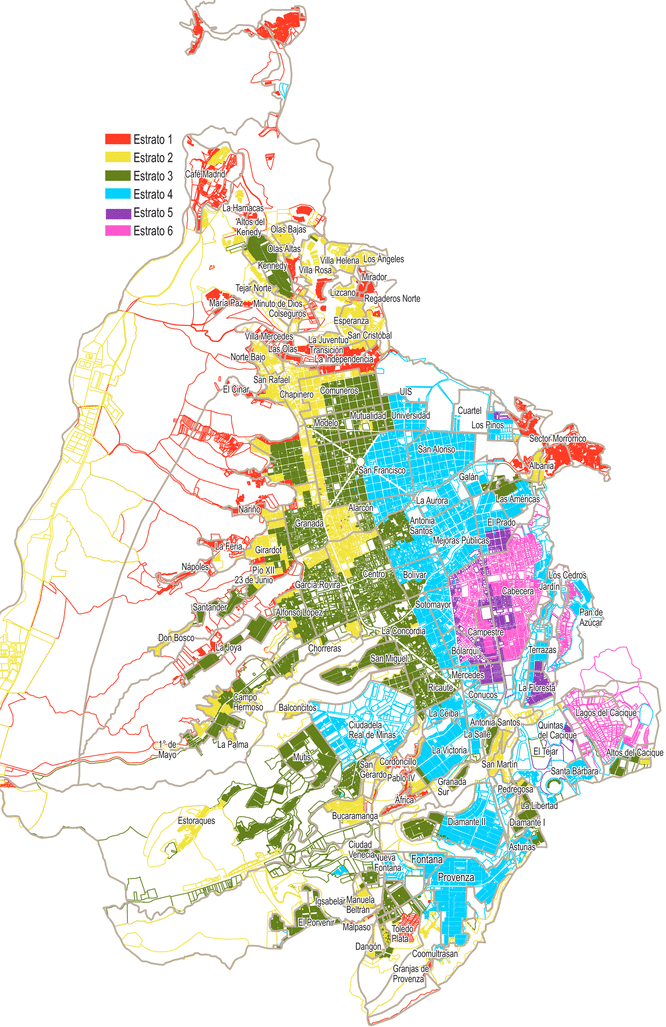
\includegraphics[width=\linewidth,height=\linewidth,keepaspectratio]{bucaramanga.png}
%     \caption{Bucaramanga}
%     \label{fig:bucaramanga}
%   \end{subfigure}%
%   \hfill
%   \begin{subfigure}{.5\textwidth}
%     \centering
%     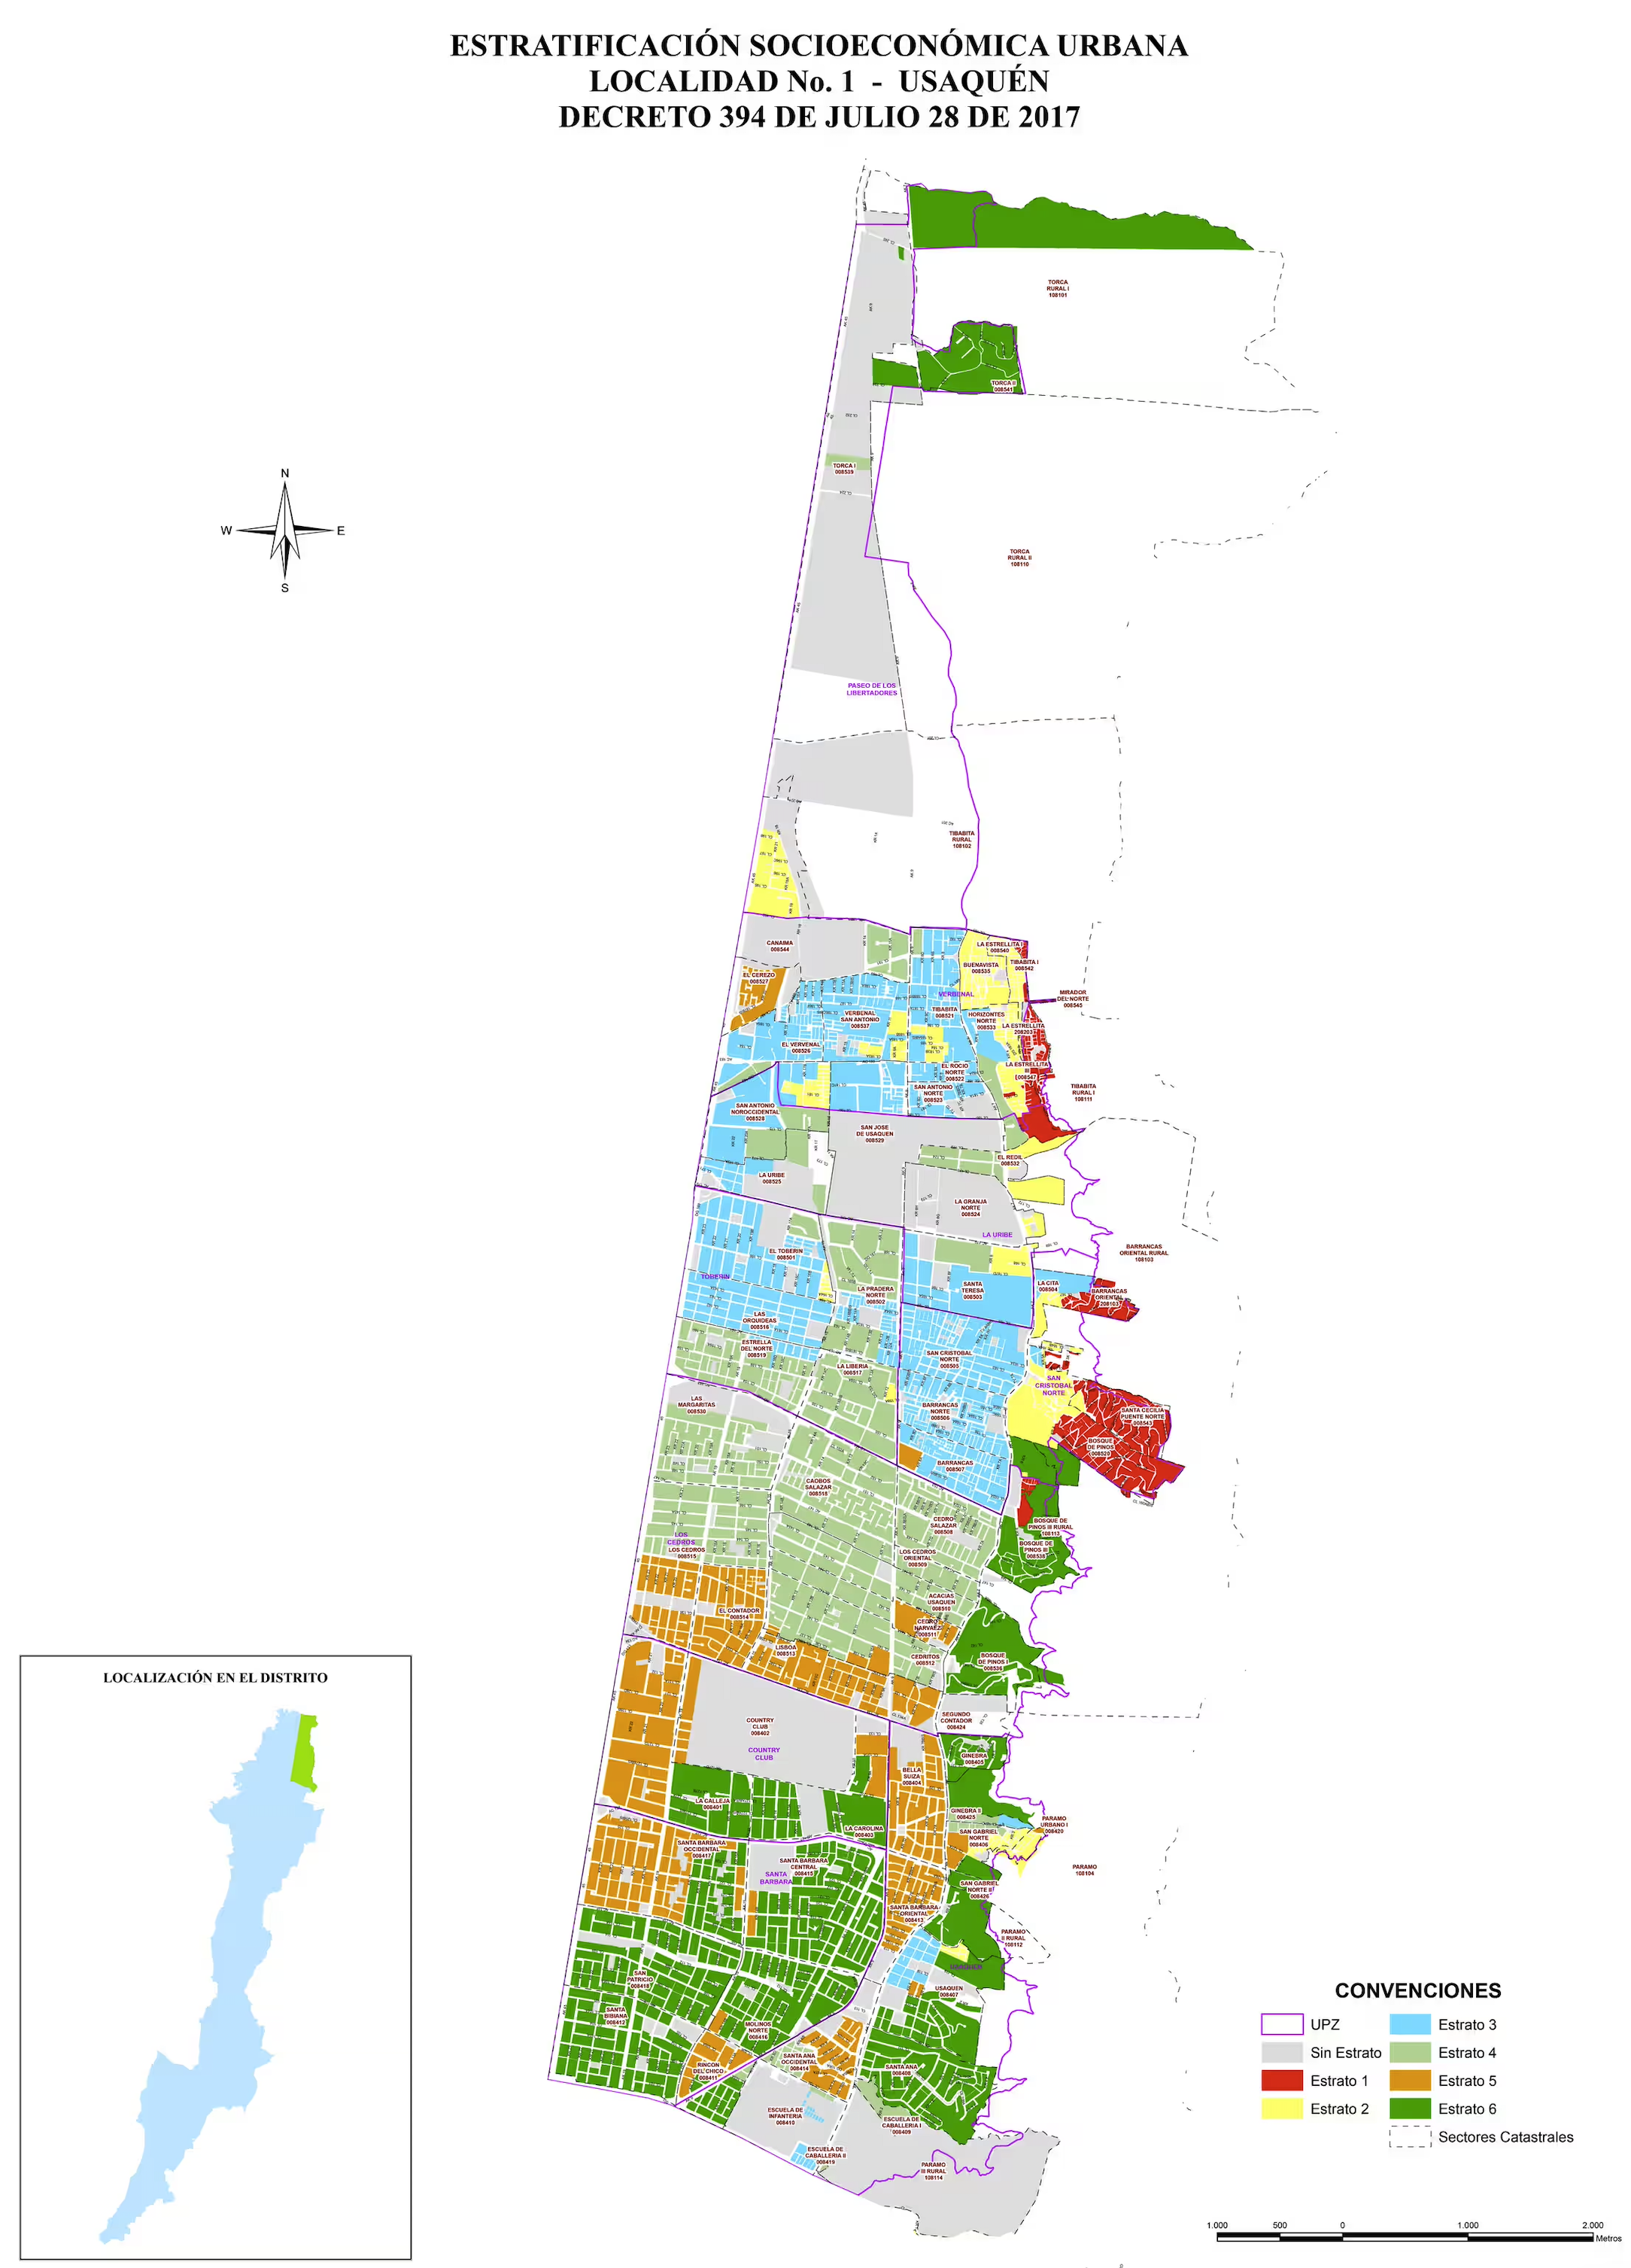
\includegraphics[width=\linewidth,height=\linewidth,keepaspectratio]{bogota.png}
%     \caption{Bogotá}
%     \label{fig:bogota}
%   \end{subfigure}
% \end{figure}


\section{Design}
We designed a referral experiment between students from different social classes, and experimentally varied the incentives to refer a low-SES peer. The study design consists of a single experiment with three sequential parts with sessions organized at the classroom level (see Figure \ref{timeline}). The instructions are provided in Appendix \ref{instructions}. 

\begin{figure}[htbp]
  \centering
  \caption{Experiment Timeline}\label{timeline}
  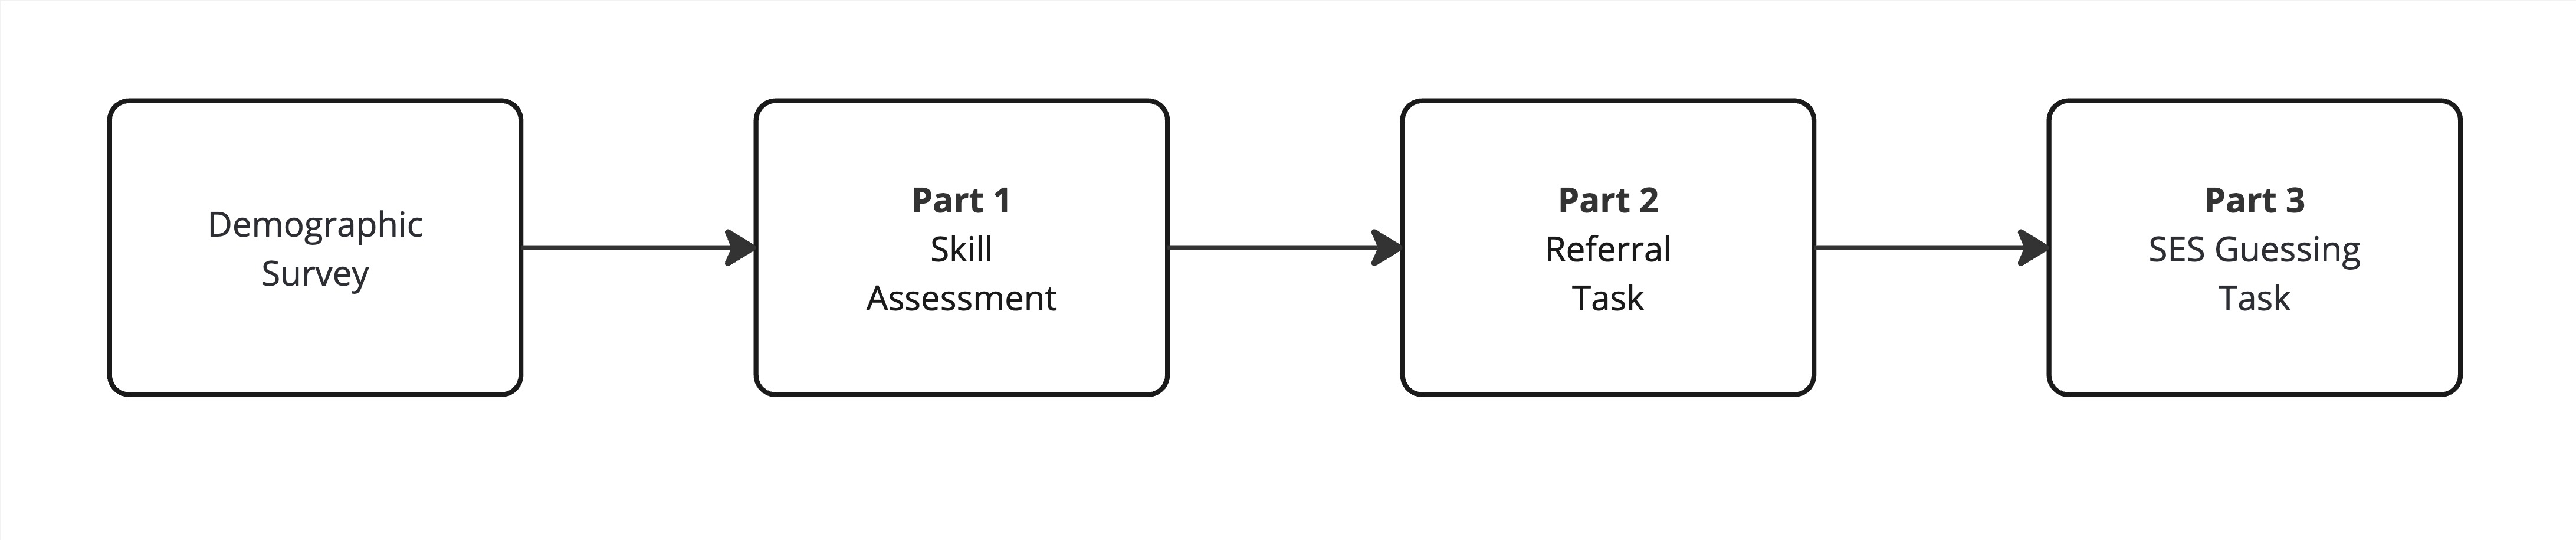
\includegraphics[width=\linewidth]{figure-1.jpg}  
  \begin{tablenotes}
\footnotesize
\item[] \textit{Note:} Participants first complete incentivized skill tests, then refer classmates for skills. In the final part, they guess the social class of their peers. This order is implemented in all sessions.
\end{tablenotes}
\end{figure}


\subsection{Skill Assessment}\label{skill_assessment}
To understand the basis for referral decisions, we collect objective measures of cognitive and social skills. These two distinct skills are crucial for the labor market and suitable in a context with university students.\footnote{For the relationship between wages and social skills conditional on cognitive skills, see \citet{kuhn2005leadership, weinberger2014increasing, deming2017growing, edin2022rising}.} This approach ensures that we observe the distribution of skills in our sample, ask for referrals on these skills, and compare how well the same individuals refer peers for a specific skill. Participants perform two incentivized skill tests. They have 5 minutes to complete each test. We provide test-specific instructions and an example item before participants begin. Correctly solved items increase chances to earn a fixed bonus.\footnote{The tests are presented in a randomized order. No performance feedback is provided. Participants see one item at a time and cannot return to previous screens once they start a test. They are not required to answer items and can skip them if they choose to do so. We elicit beliefs about performance after each test.}  \medskip\\
\textit{Cognitive Skills.} We use Raven's Progressive Matrices to measure cognitive skills \citep{raven_performances_1936, raven_standard_1976}. Raven’s test is a well-established measure of fluid intelligence, i.e., an individual’s capacity to reason and solve problems in novel situations independent of past knowledge \citep{schilbach_psychological_2016}. In this test, participants see series of images where there is a pattern with a piece that has been intentionally removed. They are tasked with choosing the piece that completes the pattern among available options. For each image, there is only one correct answer. We implement an 18-item version featuring increasingly difficult questions, with 6 response options for the first 9 items and 8 thereafter.  \medskip\\
\textit{Social Skills.} We measure social skills with the Multiracial Reading the Mind in the Eyes Test (MRMET) from \citet{kim_multiracial_2022}.\footnote{We choose MRMET because it is a race- and gender-inclusive test suitable for application in non-WEIRD (Western, Educated, Industrial, Rich, Democratic) populations like the one we sample from. The test is based on the original RMET \citep{baron-cohen_reading_2001}.} The test is an established measure for the ability to recognize emotions in others, and it has been previously used in economic experiments \citep{van_leeuwen_predictably_2018, weidmann_team_2021}. MRMET consists of photos of human faces portraying different emotions, cropped so that only the eye region is visible. Participants must choose the emotion that best describes the photo from the available answers. For each photo, there is only one correct answer and 4 response options. We administer the first 36 items in MRMET. 
% \begin{figure}[htbp]
%   \centering
%   % \captionsetup{width=0.8\linewidth}
%   \caption{Example item from the MRMET}\label{emotions-example}
%   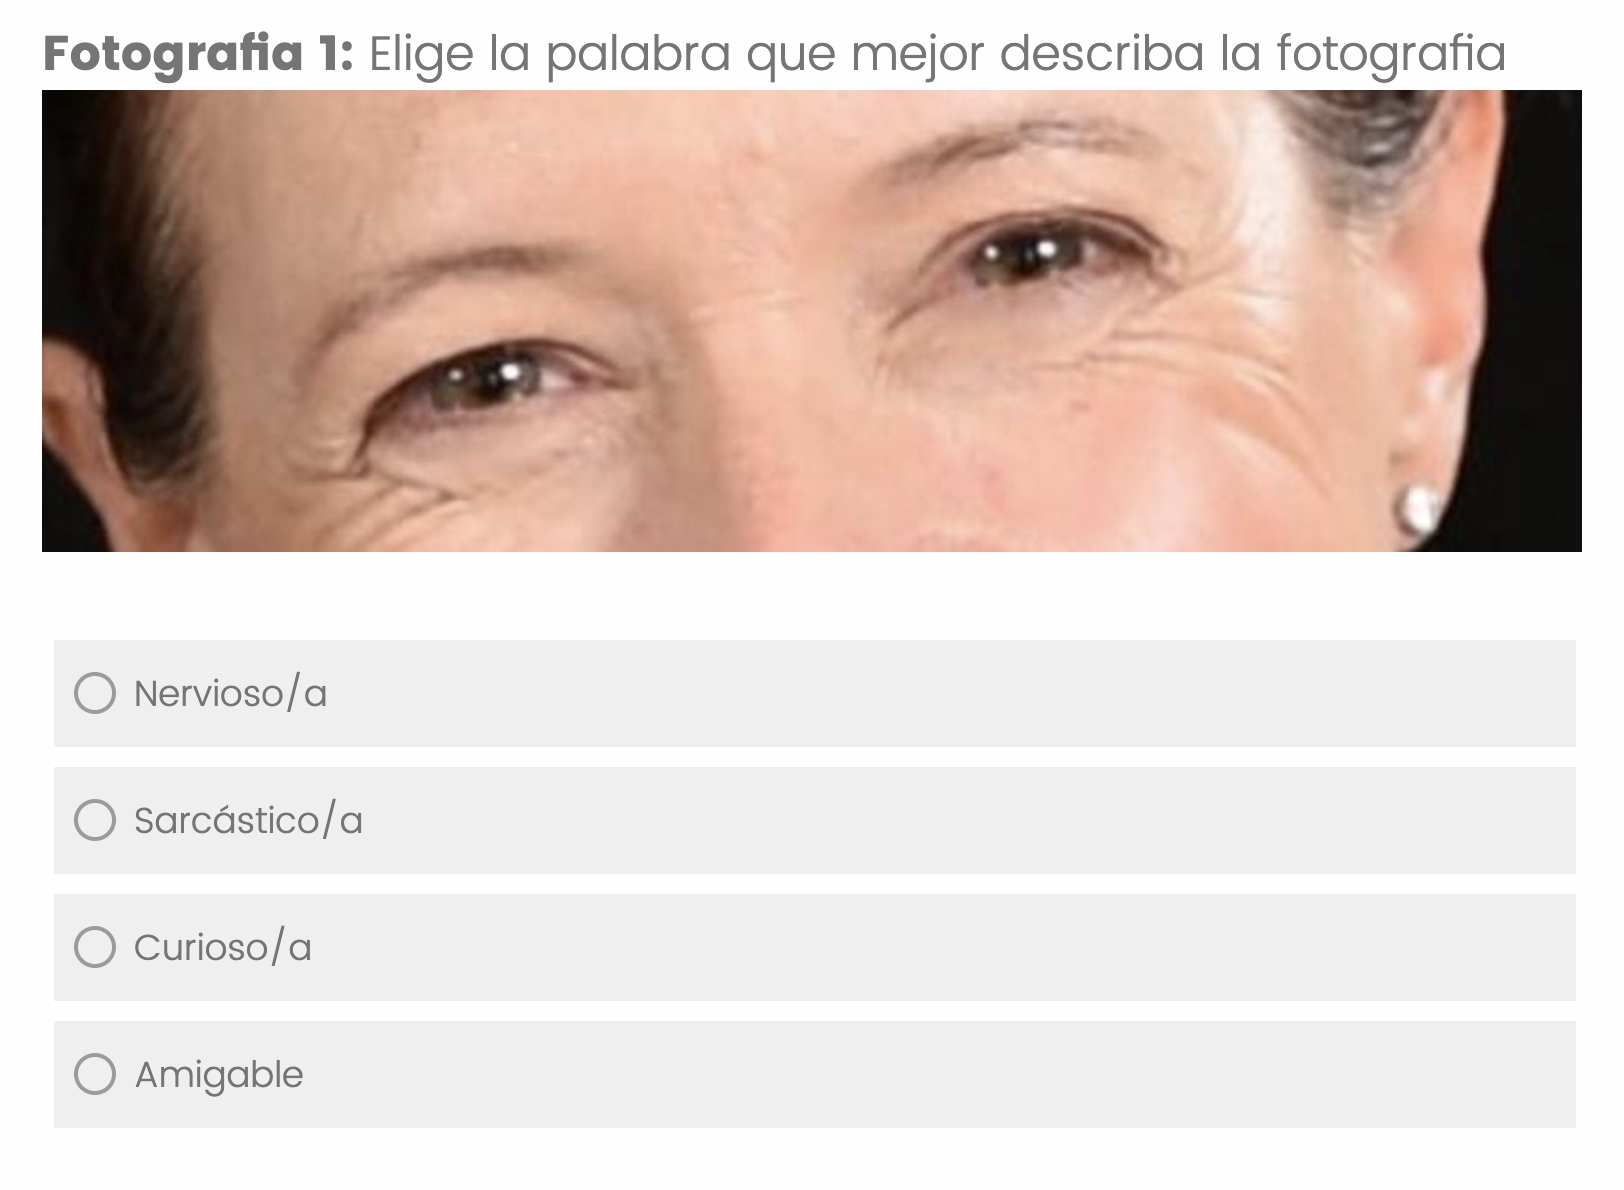
\includegraphics[scale=0.3]{social-skill-example.png}
% \end{figure}
% \begin{tablenotes}[]
% \centering
% \footnotesize
% \item[] \textit{Note:}   The correct answer for this item (translated from Spanish ``Amigable") is Friendly.
% \end{tablenotes}
\subsection{Referral Task} \label{referral_task}
We create a referral task to measure bias against low-SES peers.  For each skill, participants make incentivized referrals by nominating classmates. We first explain the measured skill accompanied by an example test item. On the following page, we provide an alphabetically ordered list of all  classmates. Using this list instead of a free text field could help alleviate biases related to recall in referral choice \textcolor{red}{cite who?}. Participants make three referral choices per skill. They are instructed to exclude themselves from referrals. A classmate may be nominated once per triad. The order in which participants refer for a skill test is randomized. We incentivize referrals with classroom-level performance rankings. The three highest-scoring classmates are designated as the top 3 for a skill. Referrers are eligible for a fixed bonus for referrals among the top 3.\footnote{We solve ties among the top 3 randomly. We describe only the top 3 selection mechanism and provide no feedback about the top 3 composition to participants.}   \medskip\\
\textit{Treatment.} We have one between subject treatment, and it varies the top 3 selection. In the \textbf{Baseline} treatment, the top 3 selection is based solely on performance ranking, regardless of other participant characteristics. The \textbf{Quota} treatment modifies the top 3 selection to prioritize low-SES individuals. We reserve the first spot in the top 3 for the highest-scoring low-SES classmate, and assign the remaining two places based on performance. This guarantees at least one low-SES participant in the top 3 per skill. Participants are informed about the top 3 selection mechanism before making referral choices (Appendix Figure \ref{fig:combined_illust} provides illustrations explaining the treatments). Assignment to the treatment is at the individual level within each classroom. This allows comparing the effect of the treatment while keeping the referral choice set constant.

\subsection{SES Guessing Task}\label{guessing_task}
Participants make guesses about the anticipated SES of their classmates. We inform participants that a computer algorithm randomly selects three students belonging to strata 1, 2, or 3. They are tasked with nominating the people they believe the computer could choose at random (Appendix Figure \ref{fig:guessing} provides the illustration explaining the task). Participants select three classmates from an alphabetically ordered list containing all their classmates. This task measures the ability to distinguish SES independent of test performance, as SES identification is relevant to our study. 
% The choice set for this task includes the participant themselves due to the specific instructions for this part. There are no time limits, but the decision time is recorded. 
\section{Sample, Incentives, and Procedure}
\textit{Sample.} We invited 849 UNAB undergraduate students to participate in the experiment. Our final sample consists of 713 individuals who completed the study protocol, resulting in an 83\% participation rate. Table \ref{tab:demographic-comparison} presents key demographic characteristics and academic performance indicators across treatments (Appendix Table \ref{tab:missing} compares the sample and missing students). The sample is well-balanced between the Baseline and Quota conditions. We observe no statistically significant differences in any of the reported variables (all \textit{p} values $> 0.1$), indicating balanced randomization. The sample is characterized by a majority of lower-SEB students. About one-third of the sample are first-generation college students. The gender distribution is balanced. The mean GPA of 3.95 is consistent across both treatments. \medskip\\ 
\textit{Incentives.} 
Participants could earn bonuses worth 100,000 Pesos (about 26 US Dollars) in each part of the experiment. In the first part, we incentivized performance in the skill tests. 20\% of participants were eligible for the bonus. We randomly picked one skill test for each eligible participant and drew a number between 1 and 100. The participant received the bonus if the percentage of correct answers in the selected test exceeded the drawn number. Chances of earning the bonus increased with each correctly solved question by 5.5\% (=1/18) for the Cognitive Skill test and by 2.78\% (=1/36) for the Social Skill test. In the second part, we incentivized referrals among the top 3 performers. 40\% of participants were eligible for the bonus. We randomly selected one skill test and one referral for each eligible participant. The participant received the bonus if their referral was among the top 3. In the third part, we incentivized the correct identification of low-SES classmates. 20\% of participants in each classroom were eligible for the bonus. We randomly selected one guess for each eligible participant. The participant received the bonus if their guess correctly identified a low-SES classmate.\medskip\\
% To mitigate potential selection bias related SEB, all invited students were enrolled in courses that combine multiple academic programs.\footnote{Previous studies at this university have shown that students from higher socioeconomic backgrounds tend to select finance and business administration programs, while those from lower socioeconomic backgrounds often choose STEM.} 
\begin{table}[!htbp]
\centering
\begin{threeparttable}
\caption{Comparison of demographic characteristics and academic outcomes across treatment conditions}
\begin{tabular*}{0.85\textwidth}{@{\extracolsep{\fill}}lcc c@{}}
\toprule
 & \multicolumn{1}{c}{\textbf{Baseline}} & \multicolumn{1}{c}{\textbf{Quota}} & \multicolumn{1}{c}{\textit{\textbf{p}}} \\ \midrule
Low-SES & 59\% & 55\% & \multicolumn{1}{c}{0.297} \\
Cognitive skill (out of 18) & 10.04 & 10.27 & \multicolumn{1}{c}{0.322} \\
Social skill (out of 36) & 18.45 & 18.50 & \multicolumn{1}{c}{0.886} \\
GPA & 3.95 & 3.95 & \multicolumn{1}{c}{0.828} \\
Entry Exam & 61.85 & 62.17 & \multicolumn{1}{c}{0.638} \\
Age & 19.33 & 19.02 & \multicolumn{1}{c}{0.228} \\
Female & 52\% & 47\% & \multicolumn{1}{c}{0.195} \\
First Generation & 34\% & 37\% & \multicolumn{1}{c}{0.386} \\
Ethnic Minority & 1\% & 3\% & \multicolumn{1}{c}{0.133} \\
Rural Community & 30\% & 27\% & \multicolumn{1}{c}{0.308} \\
Has Scholarship & 1\% & 1\% & \multicolumn{1}{c}{0.916} \\
\# Semesters at UNAB & 3.18 & 3.17 & \multicolumn{1}{c}{0.916} \\
\bottomrule
\end{tabular*}
\begin{tablenotes}[flushleft]
\footnotesize
\item[] \textit{Note:} Low-SES, Female, First Generation, Ethnic Minority, Rural, and Has Scholarship represent binary outcomes and \textit{p}-values for these variables are from two-sample tests of proportions. For continuous variables (Age, GPA, Cognitive skill, Social skill, Entry Exam, and Semester), \textit{p}-values are from two-sample t-tests with equal variances. All reported \textit{p}-values are two-tailed. Sample sizes vary slightly across measures due to missing data.
\end{tablenotes}
\label{tab:demographic-comparison}
\end{threeparttable}
\end{table}
\noindent \textit{Procedure.} Data collection occurred during the last weeks of April 2024. Our local partner, the Social Bee Lab, coordinated scheduled classroom visits and recruited research assistants to administer the experiment. Students present in class on the scheduled visit dates participated. Each classroom visit constituted a separate session.  There were in total 35 sessions. Participants accessed the Qualtrics-based experiment using their smartphones during these visits. The median time to complete the survey was 20 minutes, with a compensation of \$26 for 117 lottery winners.
% After visiting all 34 classrooms, we sent private invitations to students who were absent during the scheduled sessions. These students received the survey link via their student email and had an additional week to participate.

\section{Empirical Analysis}
\subsection{Individual Performance}
Our first goal is understanding which individuals get referred more often. Because every referrer nominates 3 classmates per skill, analyzing only the extensive margin, i.e., whether an individual gets a referral, is not very informative.\footnote{Only 86 of the 849 students (10\%) never get a referral for either skill.} We consider the fraction of referrals received by total number of referrals that could have been received instead (see Appendix Figure \ref{fig:referral_fraction} for the distribution). This approach combines the intensive and extensive margins and also makes comparisons across classrooms with different sizes easier.\footnote{The number of participating students in a classroom mechanically drives the number of total referrals that could be received by a classmate.} Our three dependent variables are fractions of: (i) cognitive skill referrals, (ii) social skill referrals, and (iii) all referrals.  

Under performance pay, higher performing classmates in skill tests should collect more referrals. However, it is not clear whether skills can be observed by referrers.\footnote{We did not provide skill feedback during the experiment. Feedback during sessions could have contaminated referral choices because participants would have incentive to share skill test results.} We therefore include other common academic performance measures that may affect our dependent variables. These measures are standardized scores of GPA and centralized entry exam to the university, similar to SAT/ACT. Regressions include $\mathbf{X}_{i}$ for all the remaining individual correlates from Table \ref{tab:demographic-comparison}. We estimate three referral fractions $y_{i}$: 
\begin{multline}
    y_{i} = \beta_0 + \beta_1{GPA}_{i} + \beta_2{E.Exam}_{i} + \beta_3{Cognitive}_{i} + \beta_4{Social}_{i} + \mathbf{X}_{i}\boldsymbol{\gamma} + \epsilon_{i}    
\end{multline}
Table \ref{tab:regression-results1} illustrates our first set of findings. Our comparison of interest is between skills and other academic performance measures. Conditional on academic performance and individual correlates specified above, there is no statistically significant difference between skill level and the fraction of referrals received for that skill (columns 1-2). This holds true also when both skills are aggregated (column 3). We emphasize aggregated fraction of referrals because most referrals overlap across skills, illustrated in Appendix Figure \ref{fig:same_}. Point estimates for skills are very close to zero. The 95\% confidence intervals rule out that a one standard deviation increase in either skill causes more than a 1 percentage point difference in the fraction of referrals received. This is an order of magnitude smaller margin when compared to the effects of a one standard deviation increase in GPA or Entry Exam. 

A one standard deviation increase in GPA increases the fraction of referrals by about 3 percentage points on a base rate of 11\% across the three dependent variables. This is a modest 27-percent increase in the fraction of referrals received.\footnote{The average participant in the average classroom with about 21 students receives 2.3 referrals. A one standard deviation increase in GPA increases this number to 2.9 referrals.} A one standard deviation increase in the Entry Exam score increases the fraction of referrals by about 2.4 percentage points for cognitive skills, with a markedly lower 1.1 percentage points for social skills. Smaller point estimates on performance metrics and lower explained variance suggests our referral model performs better for cognitive skill. Social skill referrals are seemingly made with other considerations not entirely captured in the model. The results suggest participants are not referring classmates who score high on skill tests but refer instead based on their academic performance.\footnote{Our findings are robust to: (i) restricting the observations to the baseline condition (see Appendix Table \ref{tab:regression-results-1-appendix1}), and (ii) including classroom fixed effects (Appendix Table \ref{tab:regression-results-1-appendix2}).} This may be due to classmates being able to observe academic performance of peers but not their skill test results.

% Sensitivity analysis incrementally adding academic performance measures is in Appendix Table \ref{tab:regression-results-1-appendix1-cognitive} and Table \ref{tab:regression-results-1-appendix1-social}.

\begin{table}
\centering
\begin{threeparttable}
\caption{Fraction of referrals conditional on performance and social distance}\label{tab:regression-results1}
\begin{tabular*}{0.85\textwidth}{@{\extracolsep{\fill}}l c c c@{}}
\toprule
& (1) & (2) & (3) \\
Dep. Var. & Cognitive & Social & All \\
\midrule
GPA & 0.03253\tnote{***} & 0.02759\tnote{***} & 0.03006\tnote{***} \\
& (0.00471) & (0.00494) & (0.00444) \\
Entry Exam & 0.02455\tnote{***} & 0.01113\tnote{*} & 0.01784\tnote{***} \\
& (0.00596) & (0.00583) & (0.00558) \\
Cognitive & -0.00413 & -0.00412 & -0.00413 \\
& (0.00535) & (0.00517) & (0.00499) \\
Social & 0.00267 & 0.00219 & 0.00243 \\
& (0.00414) & (0.00434) & (0.00386) \\
Constant & 0.11979\tnote{***} & 0.10607\tnote{***} & 0.11293\tnote{***} \\
& (0.04292) & (0.03959) & (0.03831) \\
\midrule
Individual Controls & Yes & Yes & Yes \\
Observations & 631 & 631 & 631 \\
R-squared & 0.162 & 0.107 & 0.147 \\
\bottomrule
\end{tabular*}
\begin{tablenotes}[flushleft]
\footnotesize
\item[] \textit{Note:} Robust standard errors in parentheses. * $p < 0.1$, ** $p < 0.05$, *** $p < 0.01$. Dependent variables are the fraction of referrals received relative to potential referrals for cognitive (1), social (2), and all referrals (3). Controls include first generation status, SES, gender, ethnicity, rural status, age, and semester. Sample is restricted to participants with complete administrative and experimental data.
\end{tablenotes}
\end{threeparttable}
\end{table}

\subsection{Social Distance}
Our second goal is understanding which individuals get referred more often, conditional on performance and social distance. As a measure of social distance between classmates, we consider the standardized fraction of classmates from the same academic program.\footnote{There is a large overlap between faculties and programs. For example, all 102 law students are in the faculty of law.Study program offers more granularity.} To address concerns about selection into courses by faculty/program we include classroom fixed effects.\footnote{Students choose when to take the two sampled mandatory courses depending on how it fits into their faculty/program-specific schedules. Since different faculties and programs have different course schedules, students cluster non-randomly into specific classes that accommodate their timetables. Without classroom fixed effects, this systematic selection pattern creates omitted variable bias in the fraction coefficients, masking the true relationship between peer availability and referral decisions.} Our dependent variable is the fraction of referrals received by total number of referrals that could have been received averaged across skills. Remaining individual correlates are included in $\mathbf{X}_{i}$. We estimate referral fraction $y_{i}$: 
\begin{multline}
    y_{i} = \beta_0 + \beta_1{GPA}_{i} + \beta_2{E.Exam}_{i} + \beta_3{Program}_{i} + \mathbf{X}_{i}\boldsymbol{\gamma} + \epsilon_{i}    
\end{multline}

\textcolor{red}{While not our main focus, one standard deviation increase in the fraction of classmates from the same academic program increases the fraction of referrals by about 1.1 percentage points across the three dependent variables (10\% increase). This effect size is comparable to the impact of the academic performance measures and considerably higher than skill test scores.}


\subsection{Social Class}
In our second empirical specification, we document whether there is social class homophily in referrals, conditional on the relevant performance measures identified earlier.\footnote{See \citet{mcpherson2001birds} for a discussion on homophily in general, for evidence on social class homophily see \citet{chetty2022social,chetty2022socialb}. For experimental evidence on a different type of homophily (gender) in referrals see \citet{beaman_job_2018}.} Specifically, we create a matched dataset between referrers and referrals for skills. We estimate social class $y_{ij}$ for referral $i$ from referrer $j$: 
\begin{multline}
    y_{ij} = \alpha + \beta_1{GPA}_{j} + \beta_2{E.Exam}_{j} + \beta_3{ReferrerSES}_{i} + \beta_4{ShareSES}_{i} + \beta_5{Program}_{i} \\ +\mathbf{X}_{i}\boldsymbol{\gamma} +  \epsilon_{i}    
\end{multline}
Our binary dependent variable takes value 1 if a referral was to a low-SES classmate and 0 otherwise. From our first specification, we include as independent variables referral GPA and entry exam scores for performance measures. Referrer SES is a dummy variable taking value 1 if the referrer is low-SES and 0 otherwise. As a measure of the SES heterogeneity in referrer choice sets, we include the fraction of low-SES classmates 



\noindent\textbf{Hypothesis 1 - Social class bias}\\
\noindent\textbf{H1a.} Does the probability of being referred depend on the social class of the potential nominees after controlling for their performance and the social class composition at the session level? In other words, is there social class bias in referrals?\\
\noindent\textbf{H1b.} Which social group makes more referrals to their own social class, controlling for performance and the social class composition at the session level? Do the lower or higher social class individuals drive the bias?

\section{hypotheses-to be removed}
\subsection{Main Analysis: Social class and referral choices across conditions}
We then examine whether the quota condition causes changes in referral compositions regarding social classes. We are also interested in understanding the equity-efficiency tradeoff of quotas, if there is one. Specifically:\\

\noindent\textbf{Hypothesis 2 - Social class quota}\\
\noindent\textbf{H2a.} Does the quota cause an increase in the number of lower social class referrals, controlling for the social class composition at the session level?  \\
\noindent\textbf{H2b.} Does the quota cause a decrease in referral quality, controlling for the social class composition at the session level? \\
\noindent\textbf{H2c.} Does the impact of the quota on referral quality and the number of lower social class referrals depend on whether the referrals are for cognitive or social skills?

\subsection{Main Analysis: Mechanisms driving bias}
We will start by looking at referral performance. Experimental evidence has shown that referrals from high-performing individuals perform better in tasks than others \citep{beaman_who_2012, beaman_job_2018,pallais_why_2016}. More precisely:\\

\noindent\textbf{Hypothesis 3 - Referrer Performance}\\
\noindent\textbf{H3a.} Do referrers with higher cognitive and/or social skills make higher quality referrals?  \\
\noindent\textbf{H3b.} Do referrers with higher cognitive and/or social skills have a smaller social class bias when making referrals?

\subsection{Exploratory Analysis}
We examine the remaining variables to complement the findings for our primary research questions. What other types of homophily do we observe in our sample? How does the referrer-referral performance correlation depend on other characteristics?     \\

\noindent\textbf{Hypothesis 4 - Additional Variables}\\
\noindent\textbf{H4a.} Does the probability of being referred depend on other characteristics of the potential nominees (e.g., age, GPA, national university entry exam score, parental education, gender, co-enrollment history, ...), controlling for performance and these characteristics at the session level? \\
\noindent\textbf{Hba.} Does the quality of referrals depend on other characteristics of the referrer (e.g., age, parental education, GPA, time spent at the university,...)? \\

\textcolor{red}{Evidence suggests social skills are harder to observe for companies \citep{bassi2022screening}. If referrers are good at discerning social skills, this could make resorting hiring via referrals a tempting choice for companies.  Referrals from high-performing individuals perform better in the same task when provided with feedback \citep{beaman_who_2012, beaman_job_2018,pallais_why_2016}. We did not provide such performance feedback to participants. Nevertheless, we had priors about how well contact would make students predict the performance of their classmates for each skill. We assumed that Cognitive skills would be easier to detect than Social skills.  With this in mind, we }


% \section{Variables}

% \subsection{General Description}
% The study begins with a demographic survey. The rest of the study is divided into three parts. Participants perform various experimental tasks designed to obtain behavioral measures in each part. Participants’ choices in these tasks are incentivized and determine their bonus earnings. In addition to the demographic survey and behavioral measures, UNAB provides complementary administrative data.

% \subsection{Demographic Survey Questions}
% \textbf{Gender.} We ask participants: ``What is your gender?" Answer options: Man, Woman.\medskip \\
% \textbf{Stratum.} We ask participants: ``What is the socio-economic stratum to which your family belongs?" Answer options range from 1 to 6. This is a government-assigned number assigned to every household in Colombia based on neighborhood-level wealth. It's a widely recognized classification system that directly affects utility costs and is visible on all utility bills. It categorizes neighborhoods into six strata, from 1 (lowest socioeconomic status) to 6 (highest socioeconomic status). Residents in higher strata pay more for utilities, while those in lower strata receive subsidies.\medskip \\
% \textbf{Parental Education.} We ask participants: ``What is the highest level of education acquired by your father (mother)?" Answer options are: Primary school, High school, Technical school, Undergraduate, Graduate, Postgraduate, Not applicable.

% \subsection{Administrative Data}
% \textbf{Co-enrollment History.} UNAB provides the co-enrollment history of participants in this study. This is a detailed list of all the classes participants have taken since their enrollment at the university, the semester during which they have taken these classes, and the classroom in which they have taken them.  \medskip \\
% \textbf{GPA.} UNAB provides the transcripts of the classes participants have taken since their enrollment at the university. \medskip\\
% \textbf{National University Entry Exam.} UNAB provides participants' scores in the national-level university entry exam that every student passes before beginning their studies in a Colombian higher education institution. \medskip\\
% \textbf{Study Program.} UNAB provides the study track of participants. \medskip\\
% \textbf{Age.} UNAB provides the age of participants.

% \subsubsection{Unincentivized Belief Elicitation}
% Participants are asked to predict their performance in the two assessment tests used to measure cognitive and social skills. After passing each test, they make a single unincentivized prediction about the relative frequency of participants who perform worse than them.\medskip\\
% \textbf{Cognitive Skills.} We ask: ``If we randomly choose 10 participants from this classroom, how many people do you think solved fewer correct problems than you?''. Answer options range from 0 to 10; participants use a slider to respond.\medskip\\
% \textbf{Social Skills.} We ask: ``If we randomly selected 10 participants from this classroom, how many people do you think solved fewer correct pictures than you?''. Answer options range from 0 to 10; participants use a slider to respond.

% \subsubsection{Skills Report}
% \textbf{Feedback Decision.} This question comes at the end of the study. We ask participants: ``Do you want to know your scores on the general intelligence test and the social skills test? We can analyze the data and give you a report that explains your strengths in these two areas. Also, what these strengths mean and how you can leverage them for personal and professional development." We also inform participants that they will be contacted for further studies if they consent. Answer options are: ``I can be contacted for new studies and to send me my report.'', ``I can be contacted to send my report, but not for new studies." ``No, I do not want to be contacted again." We collect the student email addresses of participants who agree to be contacted in the future.



% \begin{table}[]
% \centering
% \begin{tabular}{lll}
%                                        & \textbf{Baseline}     & \textbf{Quota}        \\ \cline{2-3} 
% \multicolumn{1}{l|}{\textbf{Referral}} & \multicolumn{1}{l|}{} & \multicolumn{1}{l|}{} \\ \cline{2-3} 
% \multicolumn{1}{l|}{\textbf{Guessing}} & \multicolumn{1}{l|}{} & \multicolumn{1}{l|}{} \\ \cline{2-3} 
% \end{tabular}
% \caption{2x2 factorial design}
% \label{tab1}
% \end{table}


% \section{Analyses}

% \subsection{Main Analysis: Social class and referral choices at baseline}
% We will start our analysis by examining whether belonging to the same social class predicts referral choices. In a world without bias, we should expect participants to refer based only on performance, regardless of their own and their referral's social class. In contrast, past evidence suggests we should expect homophily \citep{beaman_job_2018,bolte_role_2021, montgomery_social_1991}. Do different social classes refer to the extent of what their referrals' performance suggests?\\

% \noindent\textbf{Hypothesis 1 - Social class bias}\\
% \noindent\textbf{H1a.} Does the probability of being referred depend on the social class of the potential nominees after controlling for their performance and the social class composition at the session level? In other words, is there social class bias in referrals?\\
% \noindent\textbf{H1b.} Which social group makes more referrals to their own social class, controlling for performance and the social class composition at the session level? Do the lower or higher social class individuals drive the bias?

% \subsection{Main Analysis: Social class and referral choices across conditions}
% We then examine whether the quota condition causes changes in referral compositions regarding social classes. We are also interested in understanding the equity-efficiency tradeoff of quotas, if there is one. Specifically:\\

% \noindent\textbf{Hypothesis 2 - Social class quota}\\
% \noindent\textbf{H2a.} Does the quota cause an increase in the number of lower social class referrals, controlling for the social class composition at the session level?  \\
% \noindent\textbf{H2b.} Does the quota cause a decrease in referral quality, controlling for the social class composition at the session level? \\
% \noindent\textbf{H2c.} Does the impact of the quota on referral quality and the number of lower social class referrals depend on whether the referrals are for cognitive or social skills?

% \subsection{Main Analysis: Mechanisms driving bias}
% We will start by looking at referral performance. Experimental evidence has shown that referrals from high-performing individuals perform better in tasks than others \citep{beaman_who_2012, beaman_job_2018,pallais_why_2016}. More precisely:\\

% \noindent\textbf{Hypothesis 3 - Referrer Performance}\\
% \noindent\textbf{H3a.} Do referrers with higher cognitive and/or social skills make higher quality referrals?  \\
% \noindent\textbf{H3b.} Do referrers with higher cognitive and/or social skills have a smaller social class bias when making referrals?

% \subsection{Exploratory Analysis}
% We examine the remaining variables to complement the findings for our primary research questions. What other types of homophily do we observe in our sample? How does the referrer-referral performance correlation depend on other characteristics?     \\

% \noindent\textbf{Hypothesis 4 - Additional Variables}\\
% \noindent\textbf{H4a.} Does the probability of being referred depend on other characteristics of the potential nominees (e.g., age, GPA, national university entry exam score, parental education, gender, co-enrollment history, ...), controlling for performance and these characteristics at the session level? \\
% \noindent\textbf{Hba.} Does the quality of referrals depend on other characteristics of the referrer (e.g., age, parental education, GPA, time spent at the university,...)? \\

\bibliographystyle{apacite}
\bibliography{referrals}    

\appendix
\renewcommand{\thefigure}{A.\arabic{figure}}
\setcounter{figure}{0}

\section{Additional Figures and Tables}

\subsection{Additional Figures}
\begin{figure}[!htbp]
  \centering
  \caption{Stratum distribution of the sample}\label{strato}
  
\includegraphics[width=0.6\linewidth]{strato.png}
\end{figure}

\begin{figure}[!htbp]
  \centering
  \caption{Fraction of referrals received}\label{fig:referral_fraction}
  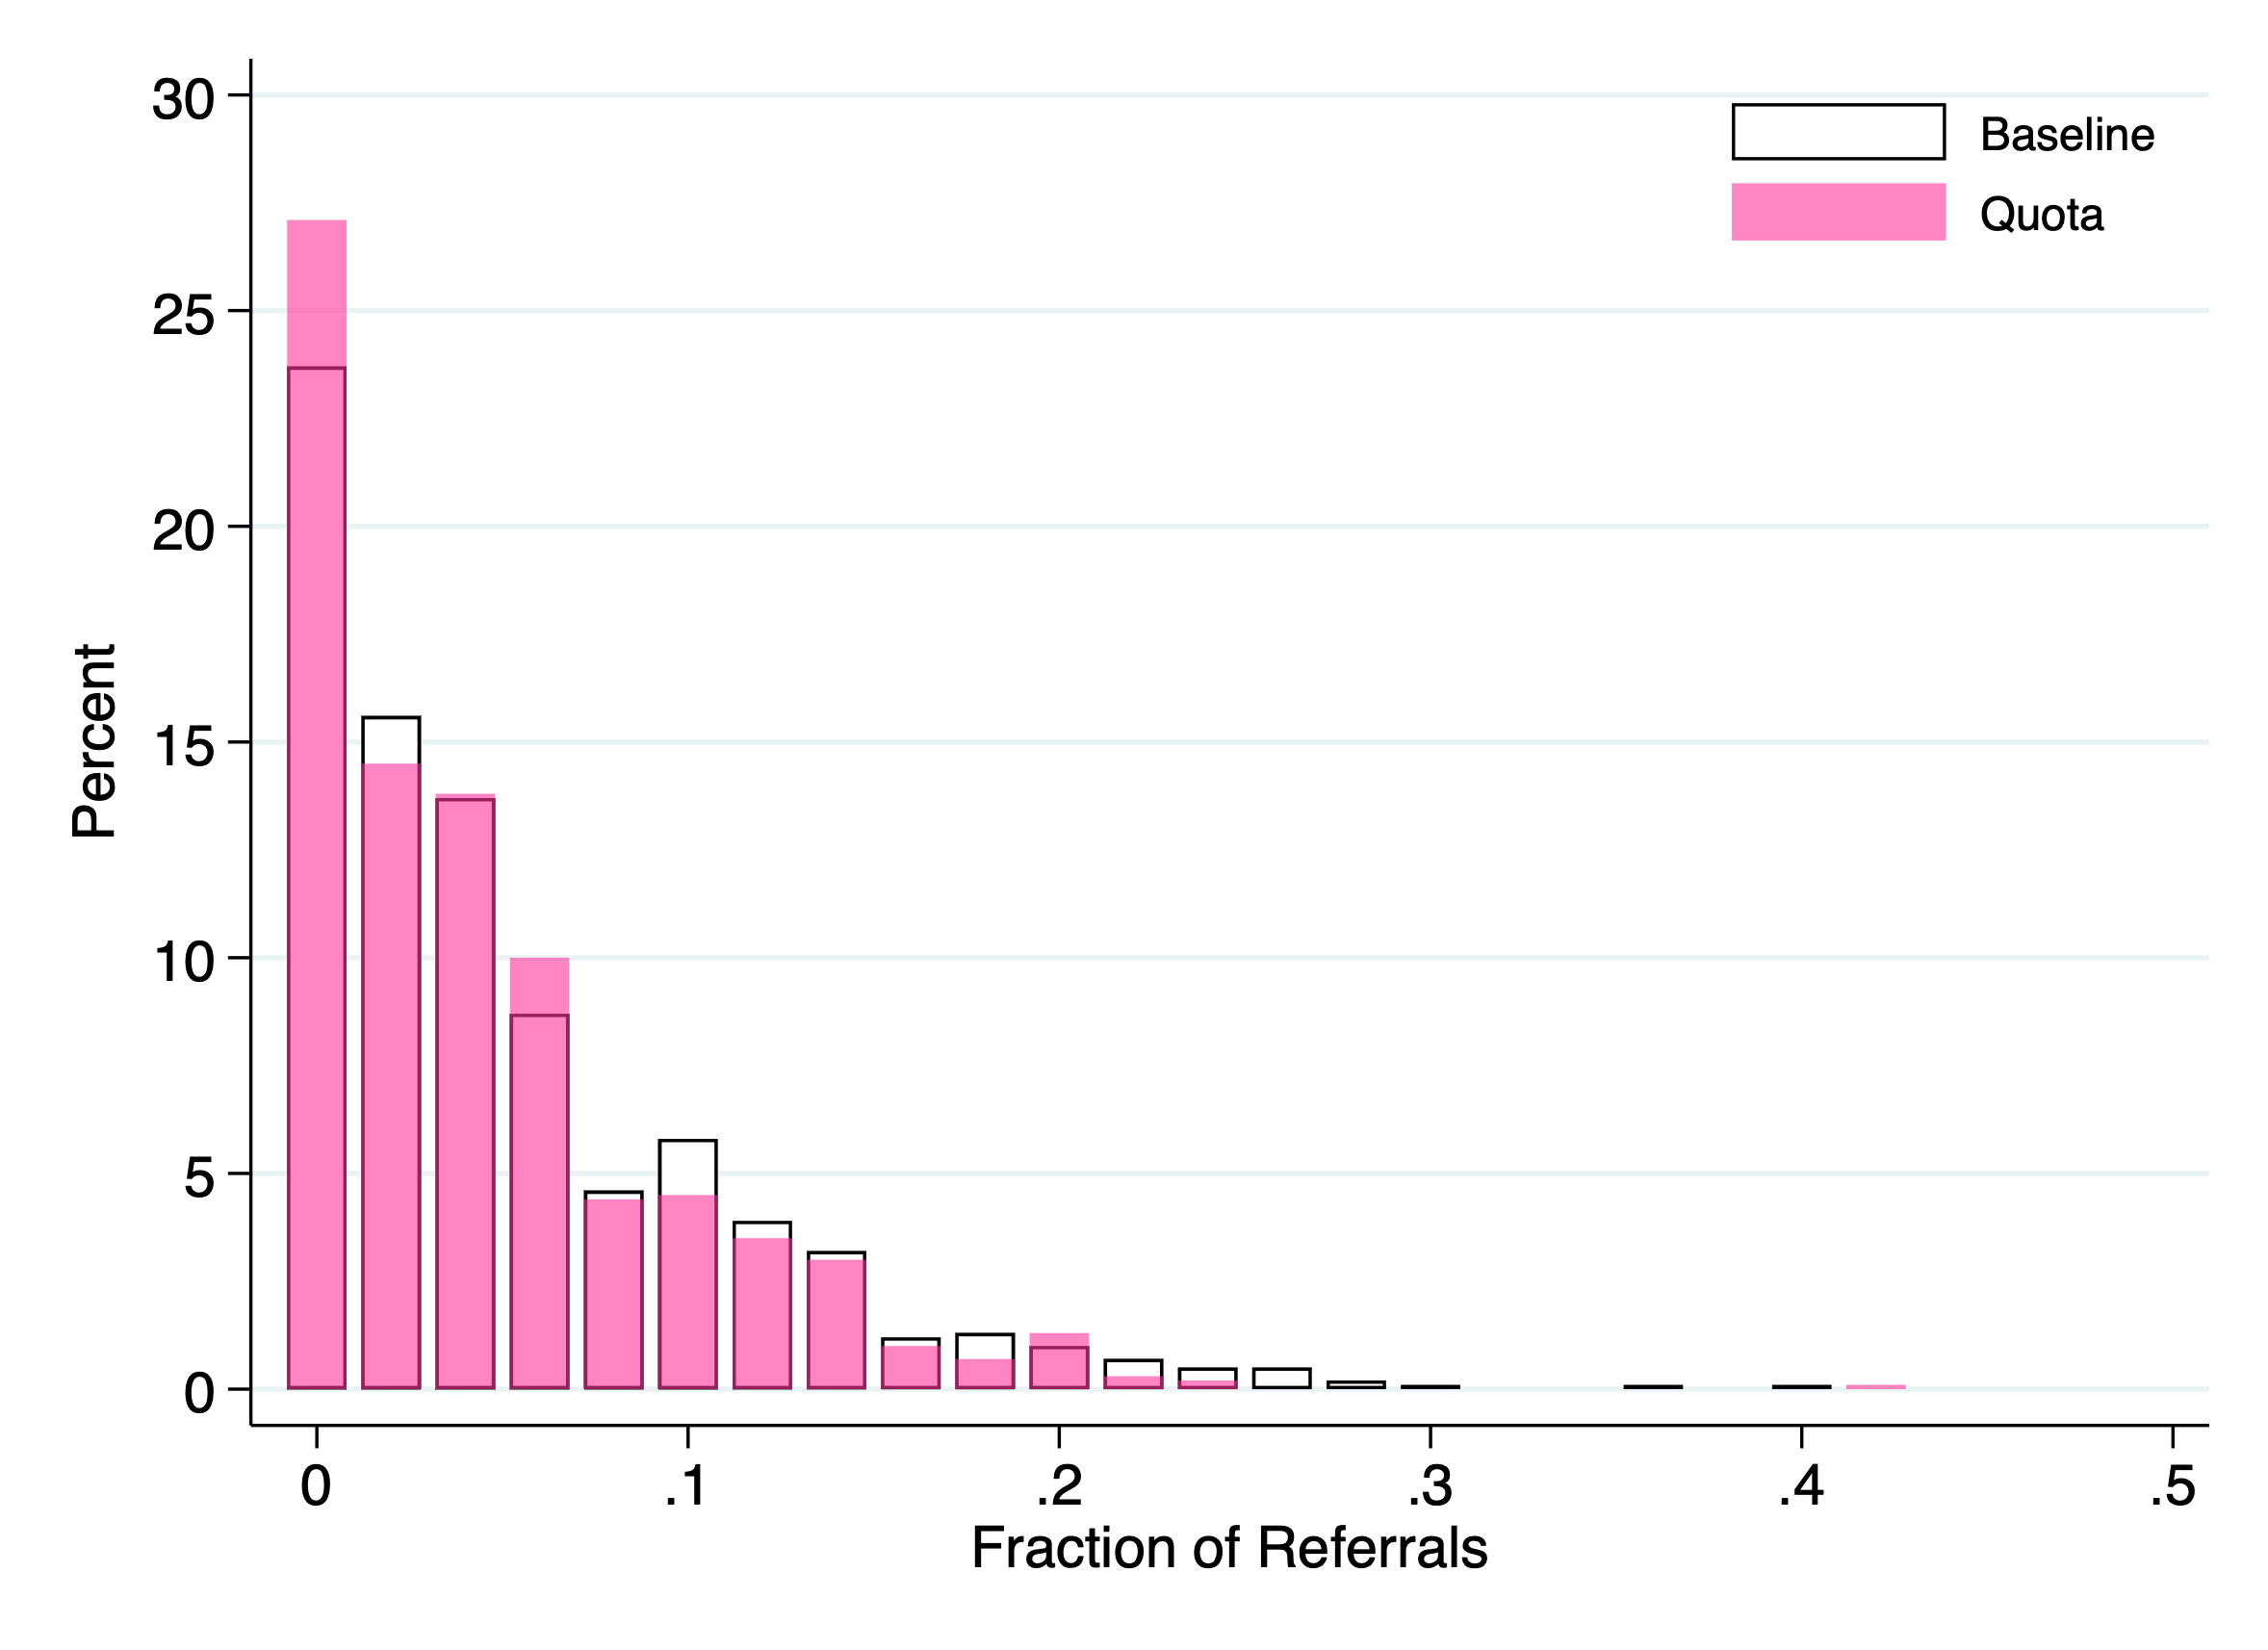
\includegraphics[width=0.6\linewidth]{referral_fraction_t1.png}
  \begin{tablenotes}
    \footnotesize
    \item[] {\textit{Note:} Fraction of referrals received for both skills by the total number of referrals that could have been received. Figure disaggregated across baseline and quota treatments.}
  \end{tablenotes}
\end{figure}

\begin{figure}[!htbp]
  \centering
  \caption{Distribution of overlapping referrals for skills}\label{fig:same_}
  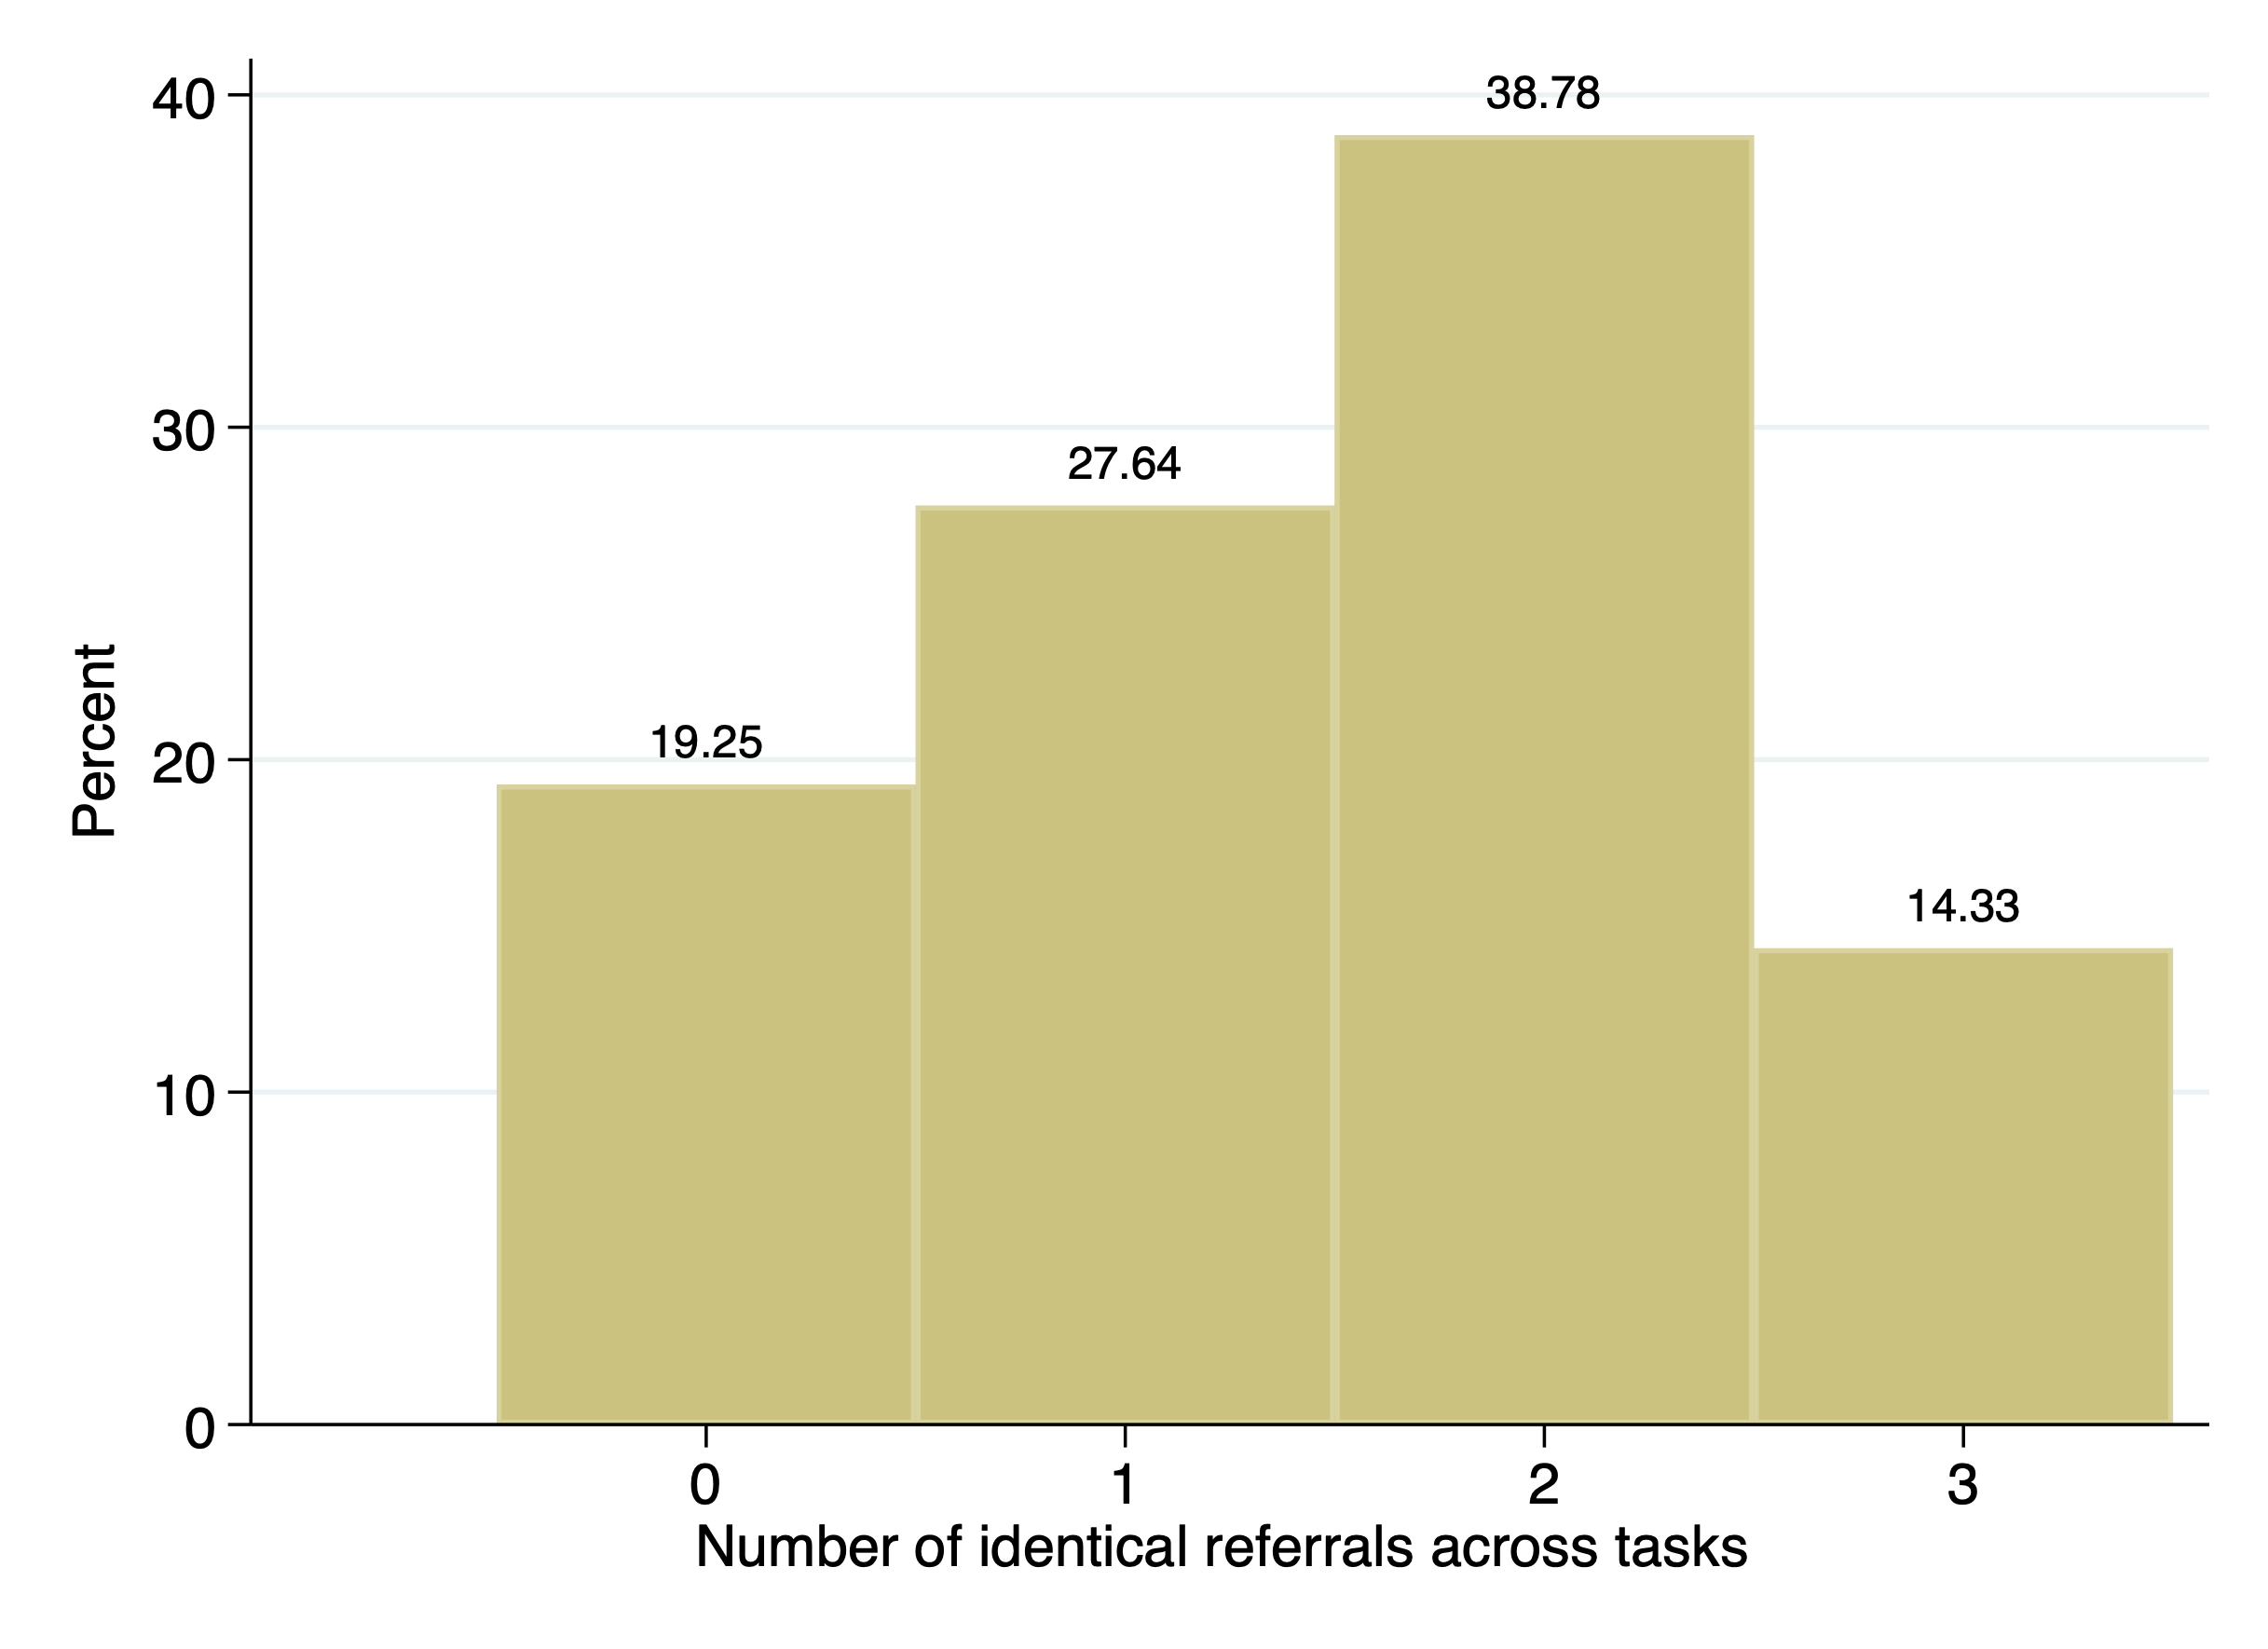
\includegraphics[width=0.6\linewidth]{same_referral.png}
  \begin{tablenotes}
    \footnotesize
    \item[] {\textit{Note:} The first bar (value of 0) indicates the percentage of individuals with all unique referrals. The last bar (value of 3) indicates the percentage of individuals with identical referral choices for both skills. Data excludes referrals that were made to one's own. Most individuals have 2 overlapping referral choices.}
  \end{tablenotes}
\end{figure}

% \begin{figure}[htbp]
%     \centering
%     \caption{Distribution of Study Programs Across Classrooms.}\label{fig:study}
%     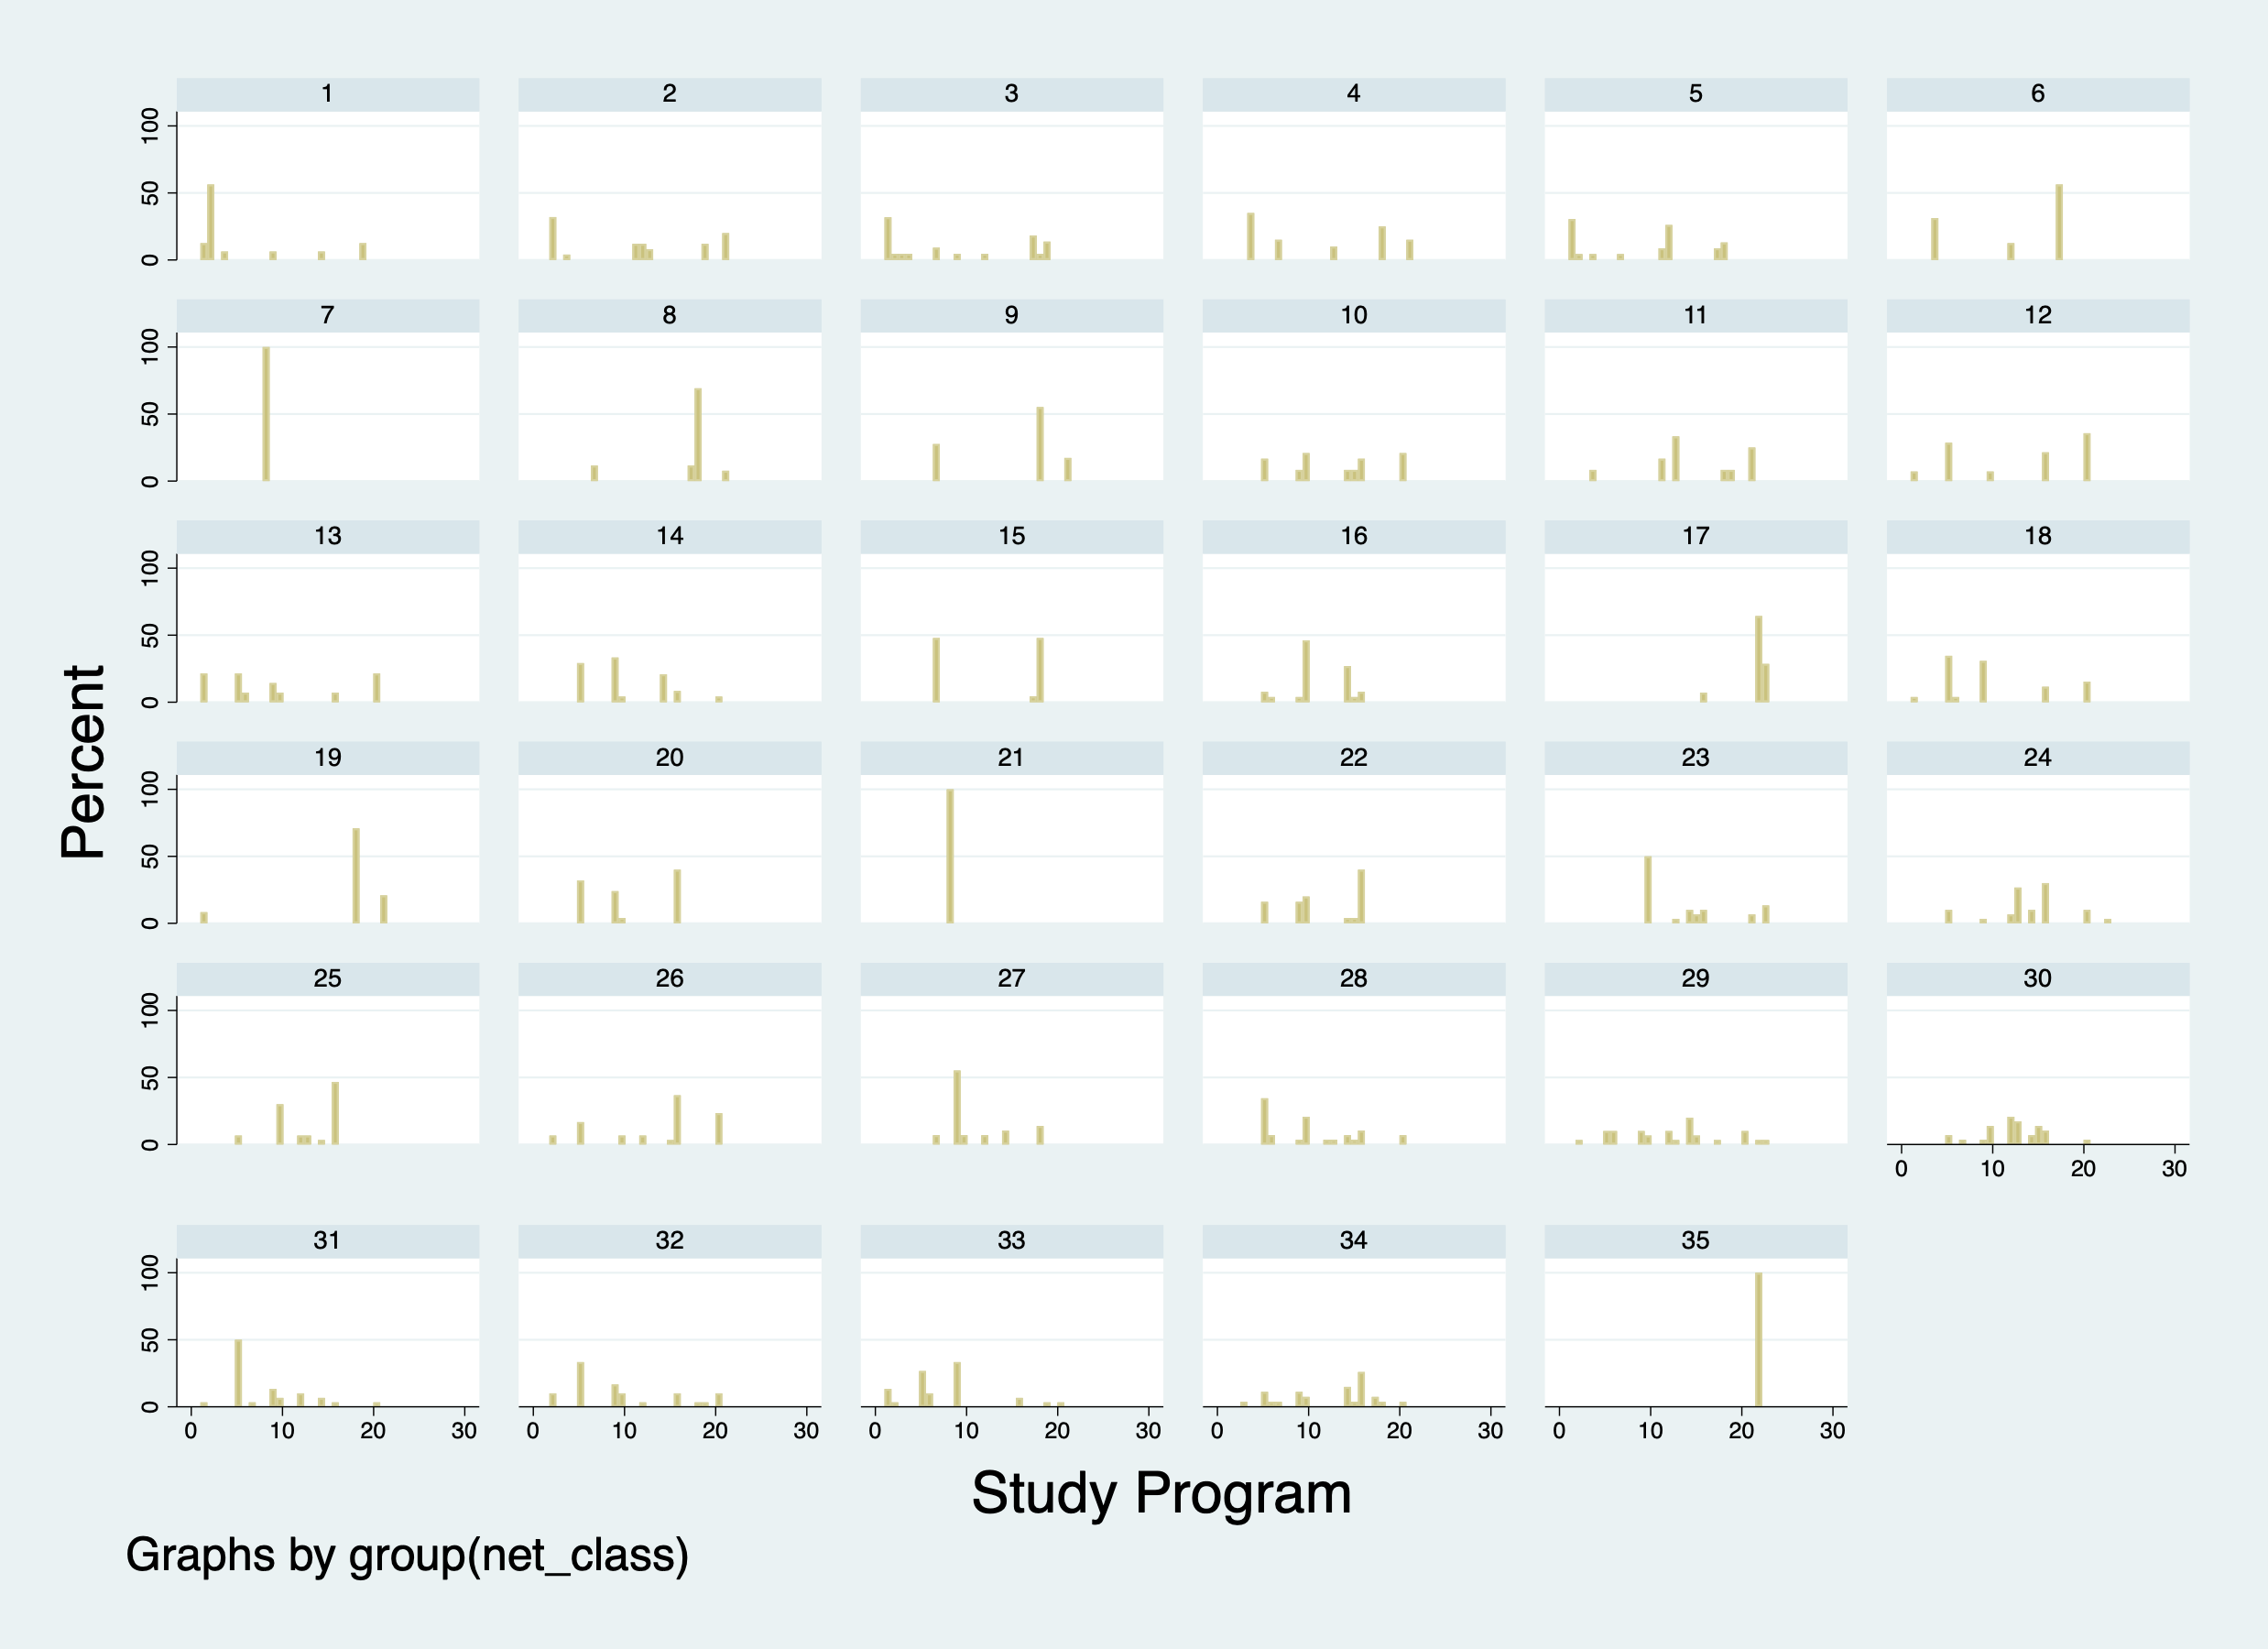
\includegraphics[width=\linewidth]{study.png}
%     \begin{tabular}{@{}c@{}}
%     \footnotesize
%     \textit{Note:} Classrooms are ordered by increasing share of low-SES individuals.
%     \end{tabular}
% \end{figure}


\subsection{Additional Tables}
\renewcommand{\thetable}{A.\arabic{table}}
\setcounter{table}{0}

\begin{table}[!htbp]
\centering
\begin{threeparttable}
\caption{Comparison of Variables Between the Sample and Missing Students}\label{tab:missing}
\begin{tabular*}{0.8\textwidth}{@{\extracolsep{\fill}}lcc c@{}}
\toprule
 & \multicolumn{1}{c}{\textbf{Sample}} & \multicolumn{1}{c}{\textbf{Missing}} & \multicolumn{1}{c}{\textit{\textbf{p}}} \\ \midrule
Ratio referrals (both skills)  & 0.127 & 0.043 & \multicolumn{1}{c}{0.000} \\
GPA (standardized) & 0.044 & -0.273 & \multicolumn{1}{c}{0.001} \\
Entry Exam (standardized) & 0.028 & -0.168 & \multicolumn{1}{c}{0.046} \\
\# Semesters at UNAB & 3.171 & 3.188 & \multicolumn{1}{c}{0.884} \\
Age & 19.182 & 20.287 & \multicolumn{1}{c}{0.001} \\
Female & 49.8\% & 48.5\% & \multicolumn{1}{c}{0.788} \\
Ethnic Minority & 2.1\% & 4.4\% & \multicolumn{1}{c}{0.114} \\
Rural Community & 28.8\% & 31.6\% & \multicolumn{1}{c}{0.501} \\
Has Scholarship & 0.8\% & 0.7\% & \multicolumn{1}{c}{0.899} \\
\bottomrule
\end{tabular*}
\begin{tablenotes}[flushleft]
\footnotesize
\item[] \textit{Note:} Values for female, ethnic minority, rural community, and scholarship represent percentages. All other variables represent means. \textit{p}-values for gender, ethnic, rural, and scholarship are from two-sample tests of proportions. For all other variables, \textit{p}-values are from two-sample t-tests with equal variances. All tests compare the sample and missing students. All reported \textit{p}-values are two-tailed.
\end{tablenotes}
\label{tab:test-results}
\end{threeparttable}
\end{table}

\begin{table}
\centering
\begin{threeparttable}
\caption{Fraction of referrals in the baseline condition conditional on performance}\label{tab:regression-results-1-appendix1}
\begin{tabular*}{0.85\textwidth}{@{\extracolsep{\fill}}l c c c@{}}
\toprule
& (1) & (2) & (3) \\
Dep. Var. & Cognitive & Social & All \\
\midrule
GPA & 0.0202\tnote{***} & 0.0180\tnote{***} & 0.0191\tnote{***} \\
& (0.0032) & (0.0030) & (0.0028) \\
Entry Exam & 0.0119\tnote{***} & 0.0056 & 0.0088\tnote{***} \\
& (0.0034) & (0.0038) & (0.0034) \\
Cognitive & 0.0003 & -0.0024 & -0.0010 \\
& (0.0031) & (0.0031) & (0.0029) \\
Social & 0.0001 & -0.0008 & -0.0004 \\
& (0.0025) & (0.0027) & (0.0023) \\
Constant & 0.0672\tnote{***} & 0.0344 & 0.0508\tnote{**} \\
& (0.0255) & (0.0239) & (0.0221) \\
\midrule
Controls & Yes & Yes & Yes \\
Observations & 631 & 631 & 631 \\
R-squared & 0.151 & 0.096 & 0.138 \\
\bottomrule
\end{tabular*}
\begin{tablenotes}[flushleft]
\footnotesize
\item[] \textit{Note:} Robust standard errors in parentheses. * $p < 0.1$, ** $p < 0.05$, *** $p < 0.01$. Dependent variables are the fraction of referrals received relative to potential referrals for cognitive (1), social (2), and all referrals (3). Controls include first generation status, SES, gender, ethnicity, rural status, age, and semester. Sample is restricted to participants with complete administrative and experimental data.
\end{tablenotes}
\end{threeparttable}
\end{table}

\begin{table}
\centering
\begin{threeparttable}
\caption{Fraction of referrals conditional on performance with classroom fixed effects}\label{tab:regression-results-1-appendix2}
\begin{tabular*}{0.85\textwidth}{@{\extracolsep{\fill}}l c c c@{}}
\toprule
& (1) & (2) & (3) \\
Dep. Var. & Cognitive & Social & All \\
\midrule
GPA & 0.0336\tnote{***} & 0.0281\tnote{***} & 0.0305\tnote{***} \\
& (0.0049) & (0.0054) & (0.0046) \\
Entry Exam & 0.0284\tnote{***} & 0.0136\tnote{**} & 0.0200\tnote{***} \\
& (0.0058) & (0.0057) & (0.0053) \\
Cognitive & -0.0043 & -0.0050 & -0.0051 \\
& (0.0050) & (0.0048) & (0.0045) \\
Social & -0.0014 & -0.0006 & -0.0001 \\
& (0.0042) & (0.0044) & (0.0039) \\
Constant & 0.1309\tnote{***} & 0.1148\tnote{***} & 0.0977\tnote{***} \\
& (0.0400) & (0.0387) & (0.0351) \\
\midrule
Classroom FE & Yes & Yes & Yes \\
Individual Controls & Yes & Yes & Yes \\
Observations & 631 & 631 & 631 \\
R-squared & 0.290 & 0.218 & 0.301 \\
\bottomrule
\end{tabular*}
\begin{tablenotes}[flushleft]
\footnotesize
\item[] \textit{Note:} Robust standard errors in parentheses. * $p < 0.1$, ** $p < 0.05$, *** $p < 0.01$. Dependent variables for columns 1 and 2 are fractions of referrals received out of all potential referrals for cognitive and social skills. Dependent variable for column 3 is the average of both skill referral fractions. Sample is restricted to participants with complete administrative and experimental data.
\end{tablenotes}
\end{threeparttable}
\end{table}

% \begin{table}
% \centering
% \begin{threeparttable}
% \caption{Fraction of cognitive skill referrals conditional on performance and social distance with incremental addition of academic performance measures}\label{tab:regression-results-1-appendix1-cognitive}
% \begin{tabular*}{0.85\textwidth}{@{\extracolsep{\fill}}l c c c@{}}
% \toprule
% & (1) & (2) & (3) \\
% Dep. Var. & Cognitive & Cognitive & Cognitive \\
% \midrule
% GPA & & 0.03593\tnote{***} & 0.03184\tnote{***} \\
% & & (0.00515) & (0.00493) \\
% Entry Exam & & & 0.02866\tnote{***} \\
% & & & (0.00588) \\
% Cognitive & 0.00854\tnote{*} & 0.00454 & -0.00394 \\
% & (0.00489) & (0.00479) & (0.00496) \\
% Social & 0.00466 & 0.00237 & -0.00129 \\
% & (0.00439) & (0.00431) & (0.00431) \\
% Program & 0.03235\tnote{***} & 0.03039\tnote{***} & 0.02859\tnote{***} \\
% & (0.00788) & (0.00755) & (0.00757) \\
% Constant & 0.12977\tnote{***} & 0.12798\tnote{***} & 0.12586\tnote{***} \\
% & (0.00422) & (0.00396) & (0.00386) \\
% \midrule
% Classroom FE & Yes & Yes & Yes \\
% Individual FE & Yes & Yes & Yes \\
% Observations & 657 & 656 & 629 \\
% R-squared & 0.2001 & 0.2743 & 0.3189 \\
% \bottomrule
% \end{tabular*}
% \begin{tablenotes}[flushleft]
% \footnotesize
% \item[] \textit{Note:} Robust standard errors in parentheses. * $p < 0.1$, ** $p < 0.05$, *** $p < 0.01$. Dependent variable is the fraction of referrals received out of all potential referrals for Cognitive skill. Sample is restricted to participants with complete administrative and experimental data.
% \end{tablenotes}
% \end{threeparttable}
% \end{table}

% \begin{table}
% \centering
% \begin{threeparttable}
% \caption{Fraction of social skill referrals conditional on performance and social distance with incremental addition of academic performance measures}\label{tab:regression-results-1-appendix1-social}
% \begin{tabular*}{0.85\textwidth}{@{\extracolsep{\fill}}l c c c@{}}
% \toprule
% & (1) & (2) & (3) \\
% Dep. Var. & Social & Social & Social \\
% \midrule
% GPA & & 0.03085\tnote{***} & 0.02801\tnote{***} \\
% & & (0.00510) & (0.00547) \\
% Entry Exam & & & 0.01361\tnote{**} \\
% & & & (0.00582) \\
% Cognitive & 0.00310 & -0.00025 & -0.00459 \\
% & (0.00445) & (0.00440) & (0.00478) \\
% Social & 0.00198 & -0.00001 & -0.00075 \\
% & (0.00436) & (0.00428) & (0.00446) \\
% Program & 0.02753\tnote{***} & 0.02574\tnote{***} & 0.02622\tnote{***} \\
% & (0.00797) & (0.00784) & (0.00814) \\
% Constant & 0.12993\tnote{***} & 0.12836\tnote{***} & 0.12765\tnote{***} \\
% & (0.00409) & (0.00388) & (0.00397) \\
% \midrule
% Classroom FE & Yes & Yes & Yes \\
% Individual FE & Yes & Yes & Yes \\
% Observations & 657 & 656 & 629 \\
% R-squared & 0.1979 & 0.2550 & 0.2622 \\
% \bottomrule
% \end{tabular*}
% \begin{tablenotes}[flushleft]
% \footnotesize
% \item[] \textit{Note:} Robust standard errors in parentheses. * $p < 0.1$, ** $p < 0.05$, *** $p < 0.01$. Dependent variable is the fraction of referrals received out of all potential referrals for Social skill. Sample is restricted to participants with complete administrative and experimental data.
% \end{tablenotes}
% \end{threeparttable}
% \end{table}

\section{Experiment}\label{instructions}
\textit{We include the English version of the instructions used in Qualtrics. Participants saw the Spanish version. Horizontal lines indicate page breaks, and clarifying comments are inside brackets.}

\noindent\rule{\textwidth}{0.4pt}\\

\noindent Please enter the password:

\noindent [classroom-specific password sent to each participant the day before data collection]

\noindent\rule{\textwidth}{0.4pt} \\

\noindent\textbf{Welcome}\\

\noindent Welcome to this study organized by the Social Bee Lab. You have been invited to participate in a survey where you can make a series of decisions. The study takes approximately 20 minutes to complete. During the study, you should not communicate with any other students. If you have any questions at any time, please raise your hand. One of the assistants will help you privately. \\

\noindent In this study, you can win bonus money depending on your choices. In total, we will draw [classroom-specific number equal to 40\% of class size] bonuses of 100.000 pesos among the participants of this classroom. It is also possible for the same person to win more than one voucher. The following screens will detail how the bonus draw will be conducted. The UNAB finance office will make the payment of the vouchers through Nequi.\\

\noindent All your decisions in this survey will be anonymized. Therefore, the answers you provide will not affect your grades in this class or your records at the university. We will use your personal information to determine the bonus allocation, but after that, we will remove any data that identifies you. \\

\noindent This survey has several parts. Each of these parts has specific instructions. Please read the instructions for each part carefully because they describe how you can earn bonuses. This study has been approved by the [omitted for anonymous review] on the condition that all the information we provide is true and all the bonuses we offer are real.\\
% Ethics Committee of New York University Abu Dhabi (NYU Abu Dhabi)
\noindent On the next screen, we present you with an informed consent form that you must accept to participate in this study.

\noindent\rule{\textwidth}{0.4pt}\\

\noindent \textbf{Informed Consent} \\ 

\noindent You have been invited to participate in a study to learn more about how people make decisions in common scenarios. \\

\noindent  This study is conducted by [omitted for anonymous review] and the Social Bee Lab at UNAB. The purpose of this study is to broaden our understanding of how people make decisions. \\

% Professor Ernesto Reuben of New York University in Abu Dhabi 

\noindent  Participation in this study is voluntary. You may opt-out at any time. No known risks are associated with your participation in this project beyond those of everyday life. Apart from the monetary bonuses that will be drawn, participation has no direct benefits.\\

\noindent  The Social Bee Lab is in charge of data collection. Your answers in this study are anonymous and will not be shared with anyone. In addition to your answers, UNAB will provide the Social Bee Lab with administrative records of your courses and your university entrance exam score. Your records, decisions, and your identity will be kept strictly confidential. Data about you collected within the scope of the study are used for scientific purposes only and are treated as strictly confidential. The Social Bee Lab will anonymize your data, and the researcher will analyze it without knowing your identity. All data generated will be stored on the researcher's computer. You have the right to access your personal data and request its deletion. You can exercise this right by contacting the researcher.\\

\noindent  If something is unclear or you have any questions, you can contact [omitted for anonymous review].\\

% Dr. Manuel Muñoz Herrera at manuel.munoz@liser.lu

\noindent  If you have questions about your rights as a participant, you can contact [omitted for anonymous review].\\

% the NYUAD IRB office at IRBnyuad@nyu.edu

\noindent  By continuing to the next screen, you agree to participate in this study.\\

\noindent\rule{\textwidth}{0.4pt}\\

\noindent Before you start, please answer these four questions. \\

\noindent What is your gender? \\ 

\noindent [Male, Female] \\

\noindent What is the socio-economic stratum to which your family belongs? \\

\noindent [Stratum 1 to Stratum 6] \\

\noindent What is your father's highest acquired level of education?\\

\noindent [Primary school, High school, Technical school, Undergraduate, Graduate, Postgraduate, Not applicable.] \\

\noindent What is your mother's highest acquired level of education?\\

\noindent [Primary school, High school, Technical school, Undergraduate, Graduate, Postgraduate, Not applicable.] \\

\noindent\rule{\textwidth}{0.4pt}\\

\noindent \textbf{Part 1} \\

\noindent You will now participate in two quizzes, each lasting five minutes. Please try to answer them to the best of your ability. \\

\noindent We will allocate up to [classroom-specific number equal to 20\% of class size] bonuses of 100.000 pesos in this first part. The steps to allocate the bonuses for Part 1 are explained below.\\

\noindent\rule{\textwidth}{0.4pt}\\

\noindent [classroom-specific illustrations explaining the incentive structure] \\

\noindent\rule{\textwidth}{0.4pt}\\

\noindent [random assignment to either cognitive or social skills test] \\

\noindent \textbf{Test - Cognitive Skill}\\

\noindent In this test, you will see a series of images. Below is an example of the images you will solve. At the top of each image, there is a pattern with a piece that has been removed. Your task is to choose which of the six pieces completes the pattern correctly. For each image, there is only one correct piece. Look at the following example: \\

\begin{figure}[htbp]
  \centering
  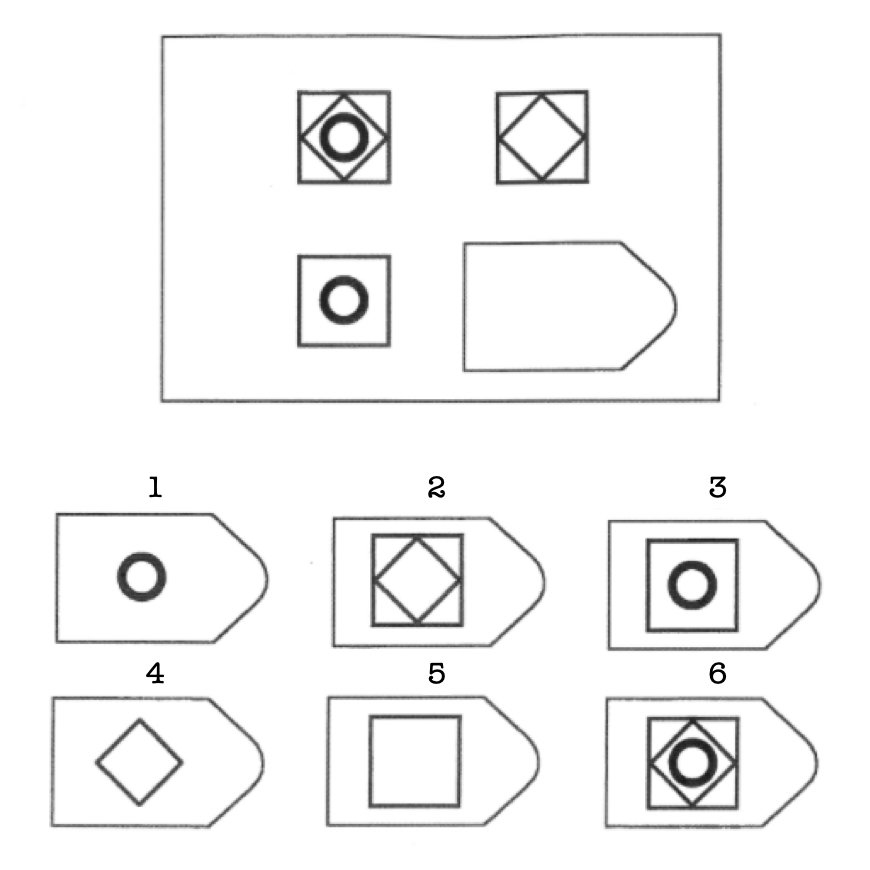
\includegraphics[scale=0.2]{Ravens Survey.jpg}
\end{figure}

\noindent First, notice a square in the upper left, the upper right, and the lower left. Also, notice that the circle is eliminated when one moves from the upper left to the upper right. Finally, the rhombus is eliminated when moving from the upper left to the lower left. Therefore, the correct piece should eliminate the circle and the rhombus, leaving only a square. So, the correct answer is piece 5. \\

\noindent To give your answer to each image, you must choose the correct option and then continue to the next screen. After giving your answer you cannot go back. \\

\noindent You will have 5 minutes to complete the test, which consists of 18 images to solve. The percentage of correct answers will determine your chances of winning one of the 100.000 pesos bonuses if you are chosen for the drawing. \\

\noindent\rule{\textwidth}{0.4pt}\\

\noindent Are you ready? \\
 
\noindent Your 5 minutes will start as soon as you move to the next screen. \\

\noindent\rule{\textwidth}{0.4pt}\\

\noindent \textbf{Problem 1}\\

\noindent [screenshot of Raven's matrix] \\

\noindent [After participants submit an answer, a new matrix appears on the screen. The sequence of matrices is the same for all participants. Participants cannot return to a previous screen. Participants do not have to provide answers for all 18 matrices.] \\

\noindent\rule{\textwidth}{0.4pt}\\

\noindent You have finished the test. You can proceed to the next screen. \\

\noindent\rule{\textwidth}{0.4pt}\\

\noindent \textbf{How did you do on the test?} \\

\noindent If we randomly choose 10 participants from this classroom, how many people do you think solved fewer correct problems than you?\\

\noindent [Slider from 0 to 10]\\

\noindent\rule{\textwidth}{0.4pt}\\

\noindent \textbf{Test - Emotions} \\
 
\noindent In this test, you will see a series of photographs. Below is an example of the pictures you will see. In each picture, you will see the eyes of a person. Below the picture, you will see four possible emotions that this person is feeling. Your task is to choose which of the four emotions correctly describes what the person is feeling. For each picture, there is only one emotion. Look at the following example: \\

\begin{figure}[htbp]
  \centering
  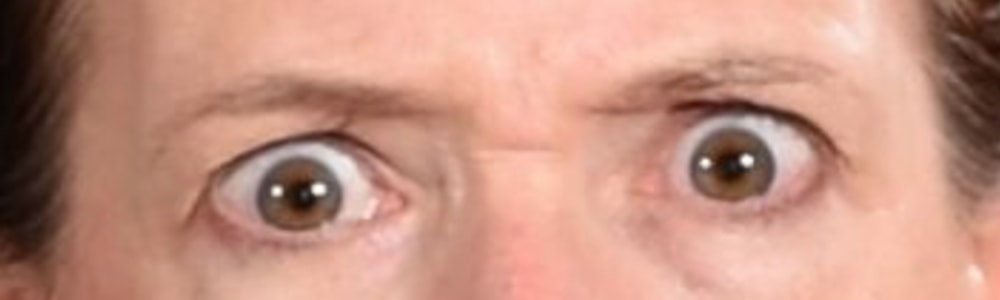
\includegraphics[scale=0.2]{3Aghast-J.jpg}
\end{figure}

\noindent [Happy, Disappointed, Shocked, Worried] \\

\noindent In this case, the correct answer is: Shocked. \\

\noindent To give your answer to each picture, you must choose the correct option and then continue to the next screen. After giving your answer you will not be able to go back. \\

\noindent You will have 5 minutes to complete the test, which consists of 36 photographs to solve. The percentage of correct answers you get will determine your chances of winning one of the 100.000 pesos bonuses if you are chosen for the drawing. \\

\noindent\rule{\textwidth}{0.4pt}\\

\noindent Are you ready? \\
 
\noindent Your 5 minutes will start as soon as you move to the next screen. \\

\noindent\rule{\textwidth}{0.4pt}\\

\noindent \textbf{Photograph 1: Choose the word that best describes the photograph} \\

\noindent [photo from Multiracial Reading the Mind in the Eyes Test] \\

\noindent [After participants submit an answer, a new photo appears on the screen. The sequence of photos is the same for all participants. Participants cannot return to a previous screen. Participants do not have to provide answers for all 36 photos.] \\

\noindent\rule{\textwidth}{0.4pt}\\

\noindent You have finished the test. You can proceed to the next screen. \\

\noindent\rule{\textwidth}{0.4pt}\\

\noindent \textbf{How did you do on the test?} \\

\noindent If we randomly choose 10 participants from this classroom, how many people do you think solved fewer correct photographs than you?\\

\noindent [Slider from 0 to 10]\\

\noindent\rule{\textwidth}{0.4pt}\\

\noindent \textbf{Part 2} \\
 
\noindent At the beginning of this study, all participants took two tests, one on cognitive ability and one on emotions. In this part, we will ask you to recommend the people who in your opinion will score the best on each test. \\

\noindent You may recommend 3 people per test, but you may not recommend yourself. \\

\noindent We will allocate up to [classroom-specific number equal to 40\% of class size] bonuses of 100.000 pesos for Part 2. The steps for allocating bonuses are explained below. \\

\noindent\rule{\textwidth}{0.4pt}\\

\noindent [random assignment to either quota or baseline condition] \\

\noindent [classroom-specific illustrations explaining the incentive structure depending on assignment to either baseline or quota conditions] \\


\begin{figure}[!htbp]
  \centering
  \caption{Illustrations for the two conditions}
  \begin{subfigure}[b]{0.48\textwidth}
    \centering
    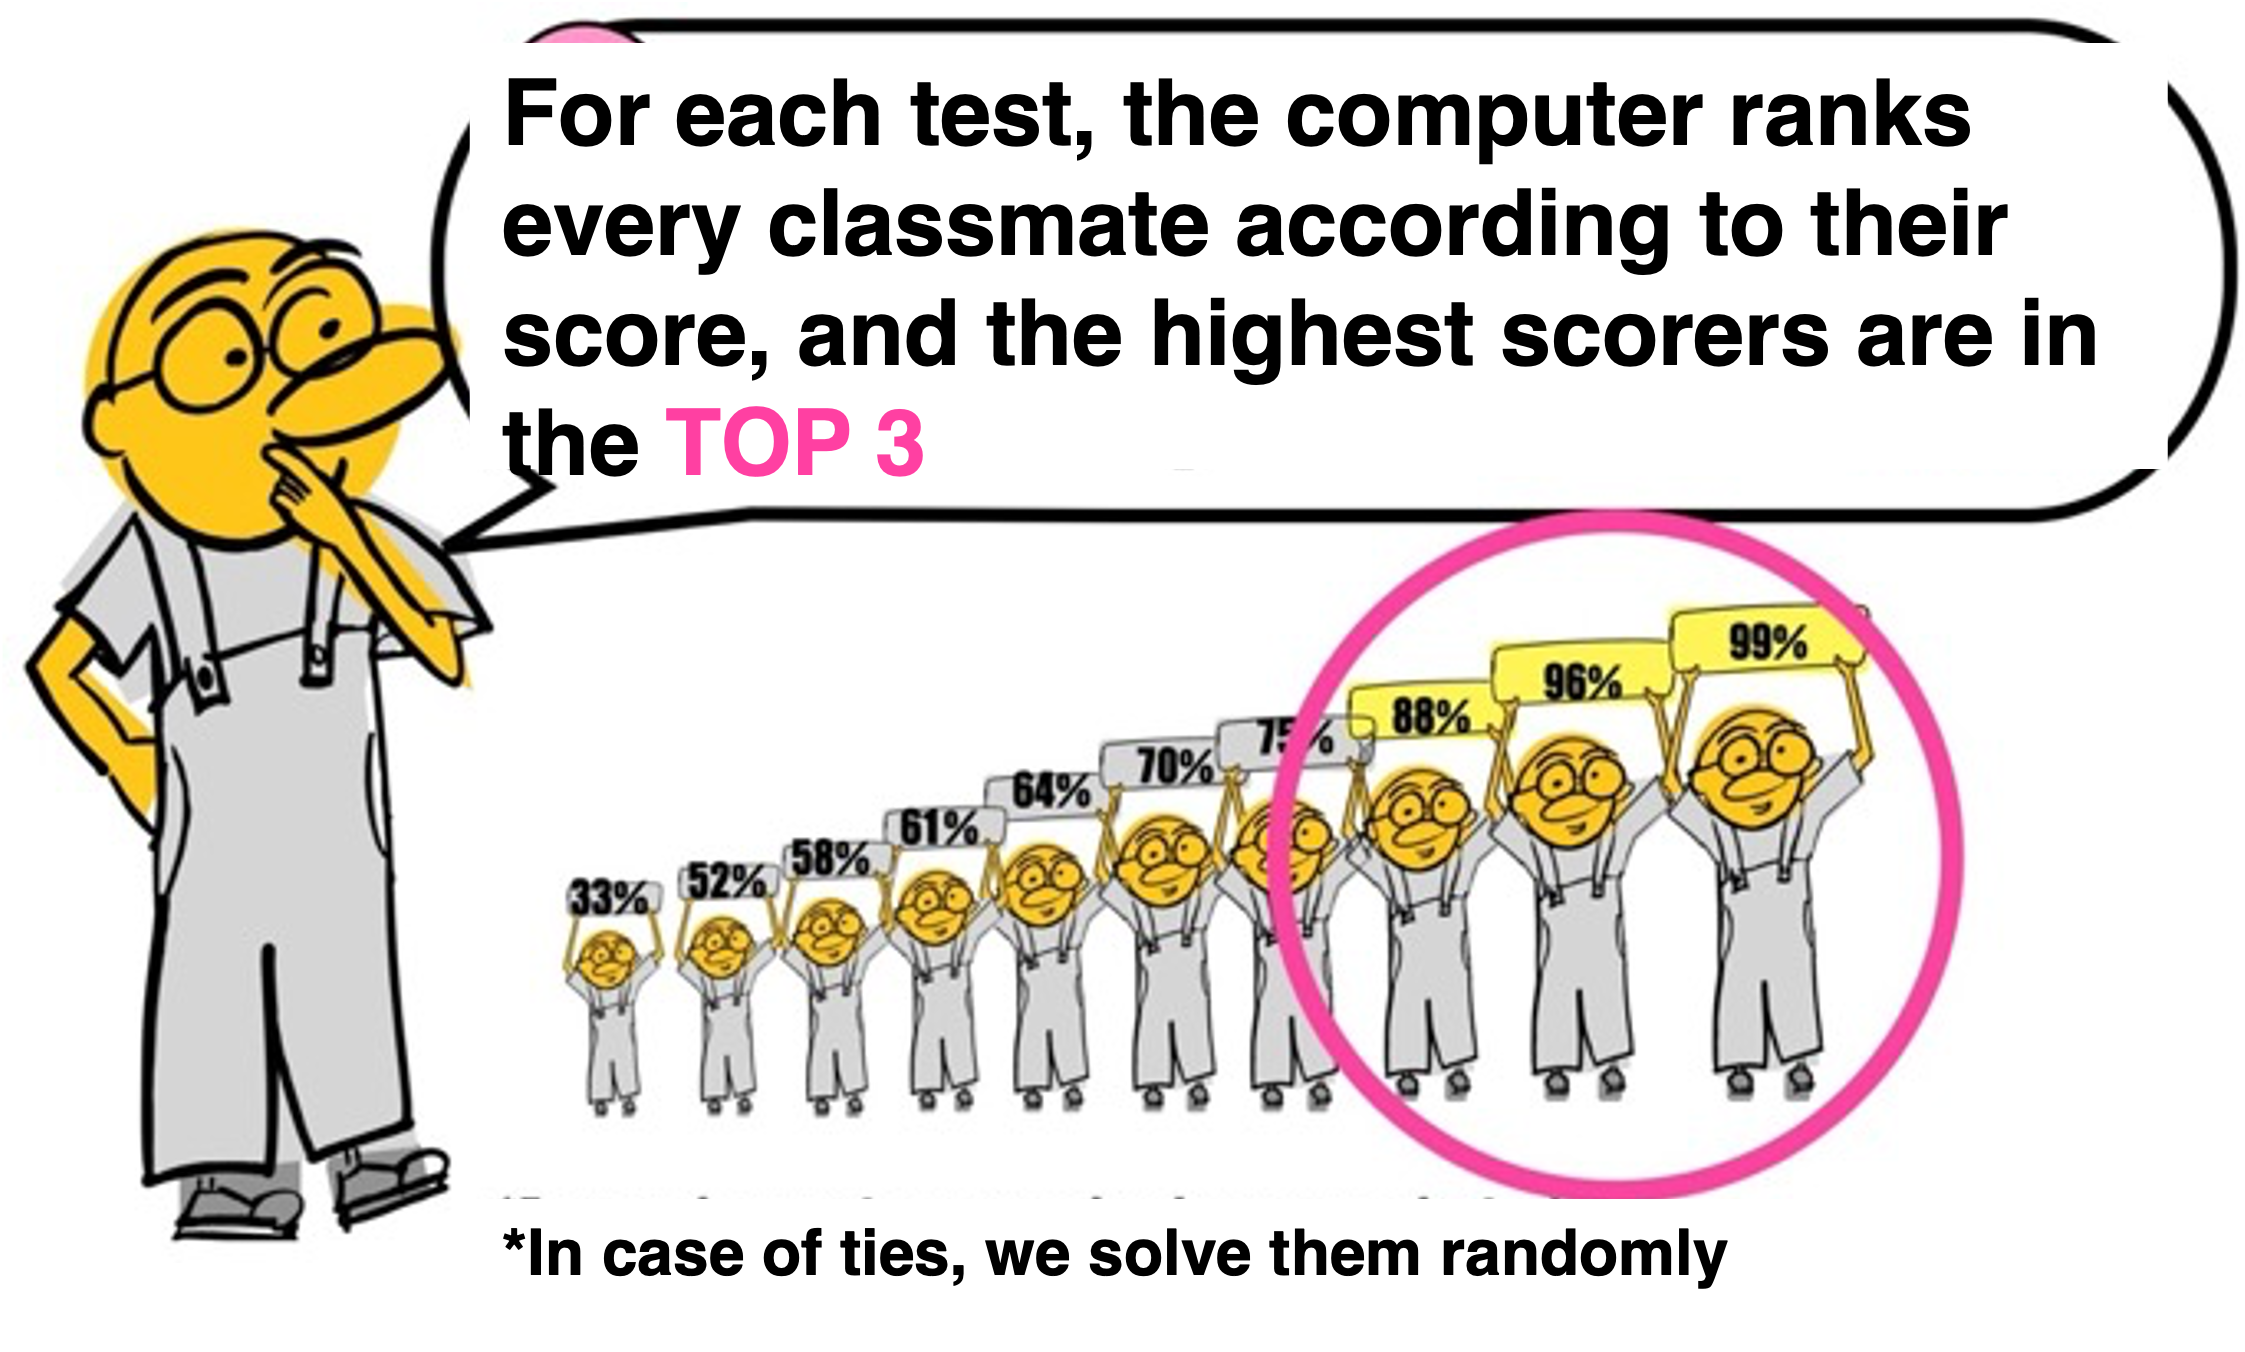
\includegraphics[width=\textwidth]{baseline.png}
    \caption{Baseline}
    \label{baseline_illust}
  \end{subfigure}
  \hfill
  \begin{subfigure}[b]{0.48\textwidth}
    \centering
    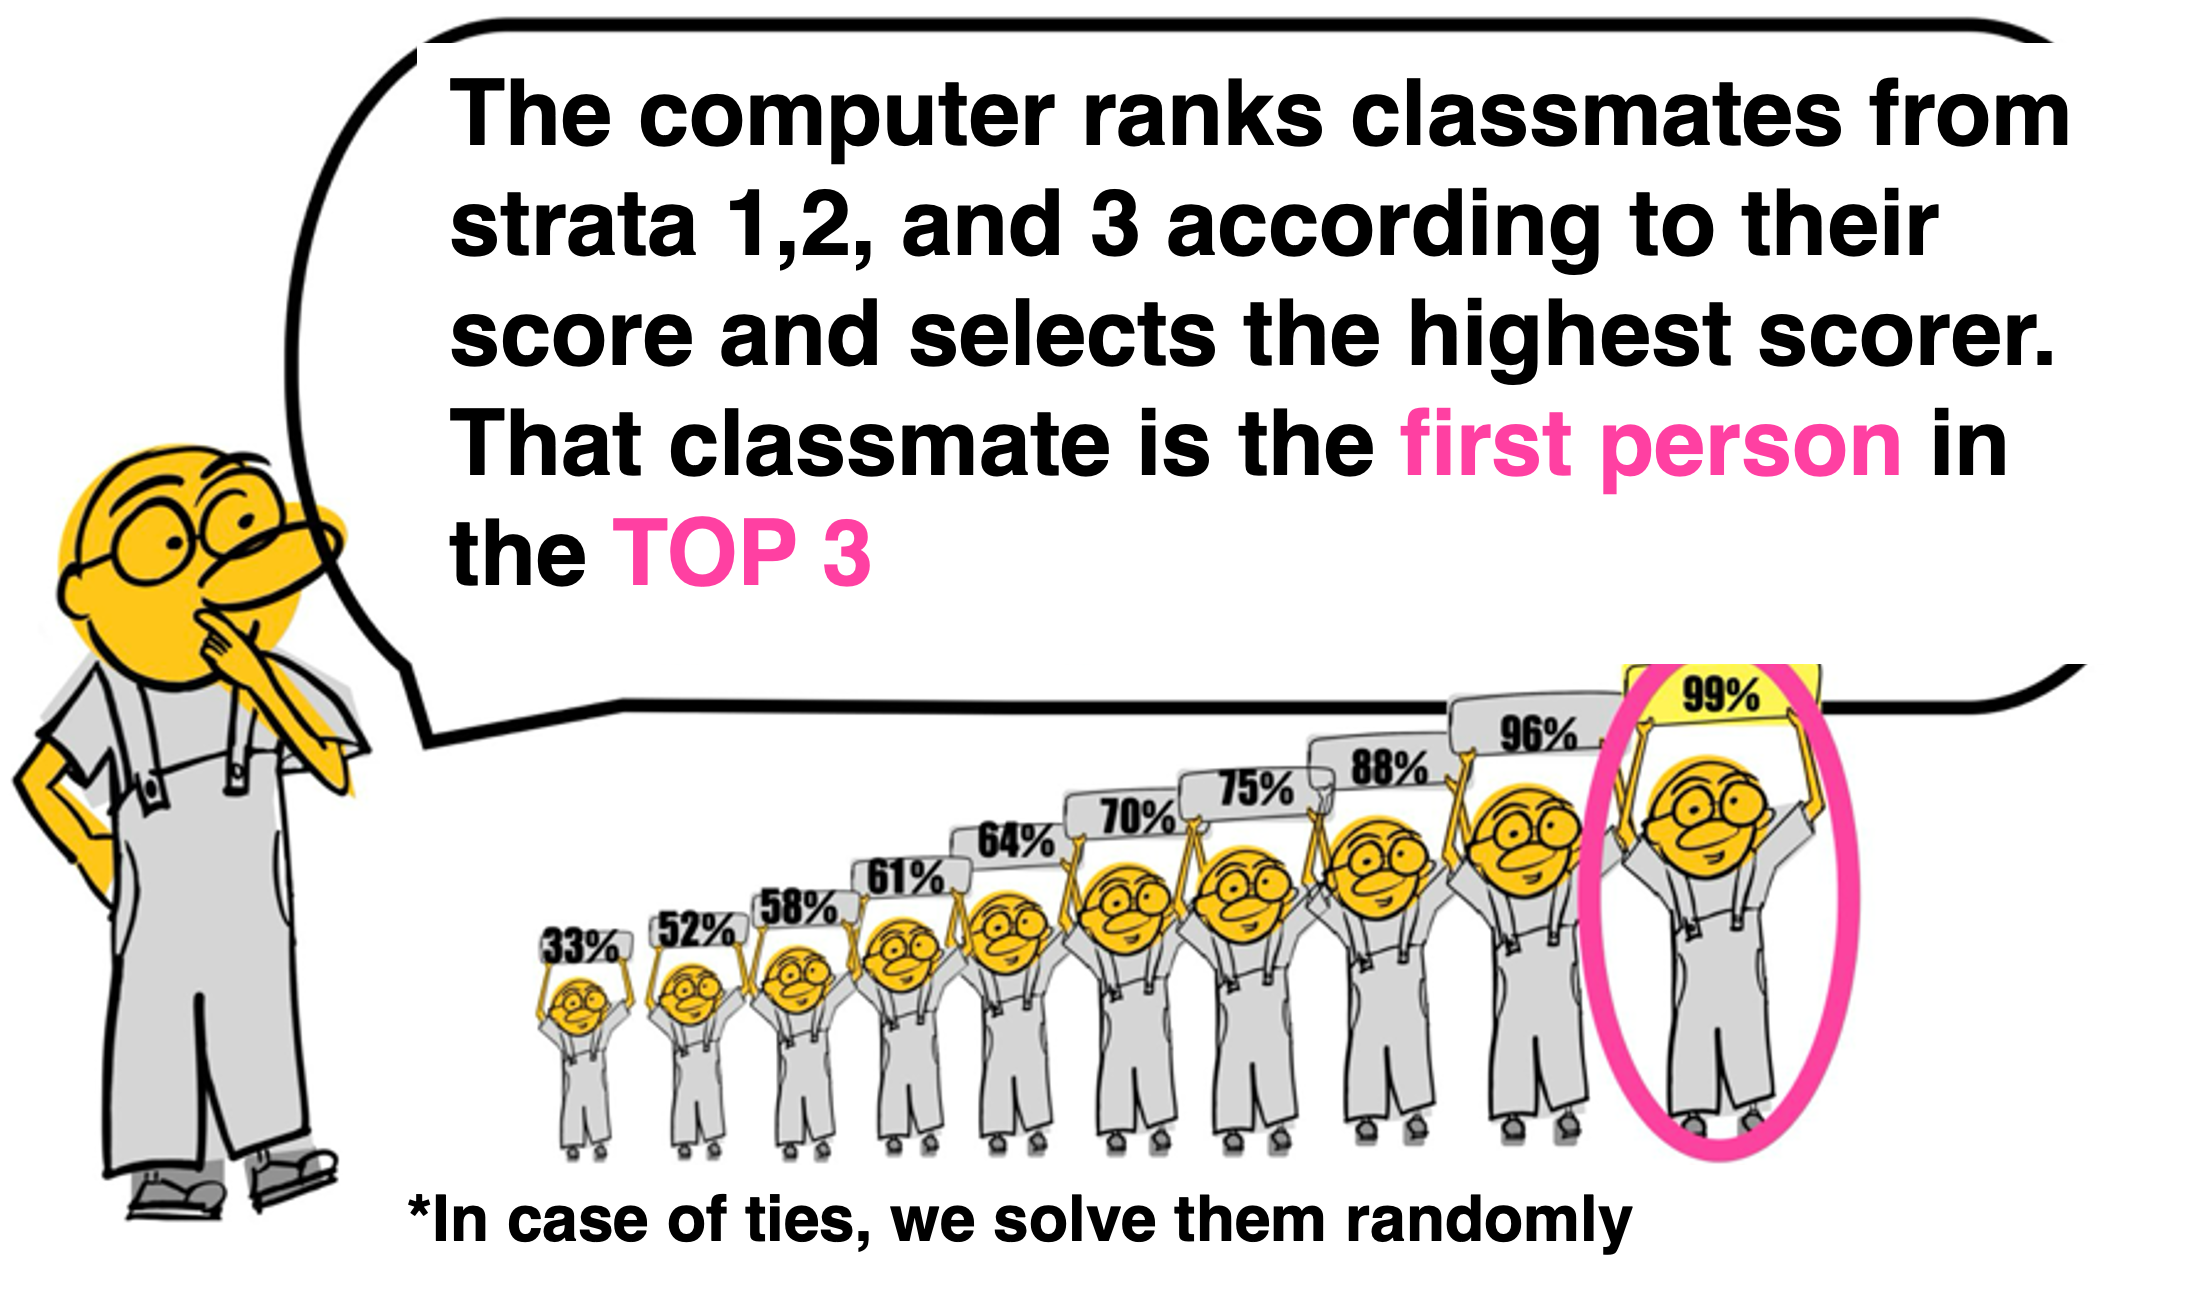
\includegraphics[width=\textwidth]{quota.png}
    \caption{Quota}
    \label{quota_illust}
  \end{subfigure}
  \label{fig:combined_illust}
\end{figure}

\noindent\rule{\textwidth}{0.4pt}\\

\noindent [random assignment to either cognitive or social skills referral task] \\

\noindent \textbf{Recommendation - Cognitive Skill}\\

\noindent All participants took a test to identify the missing pattern in each image, as in the example below. This test is used to measure general intelligence.\\

\begin{figure}[htbp]
  \centering
  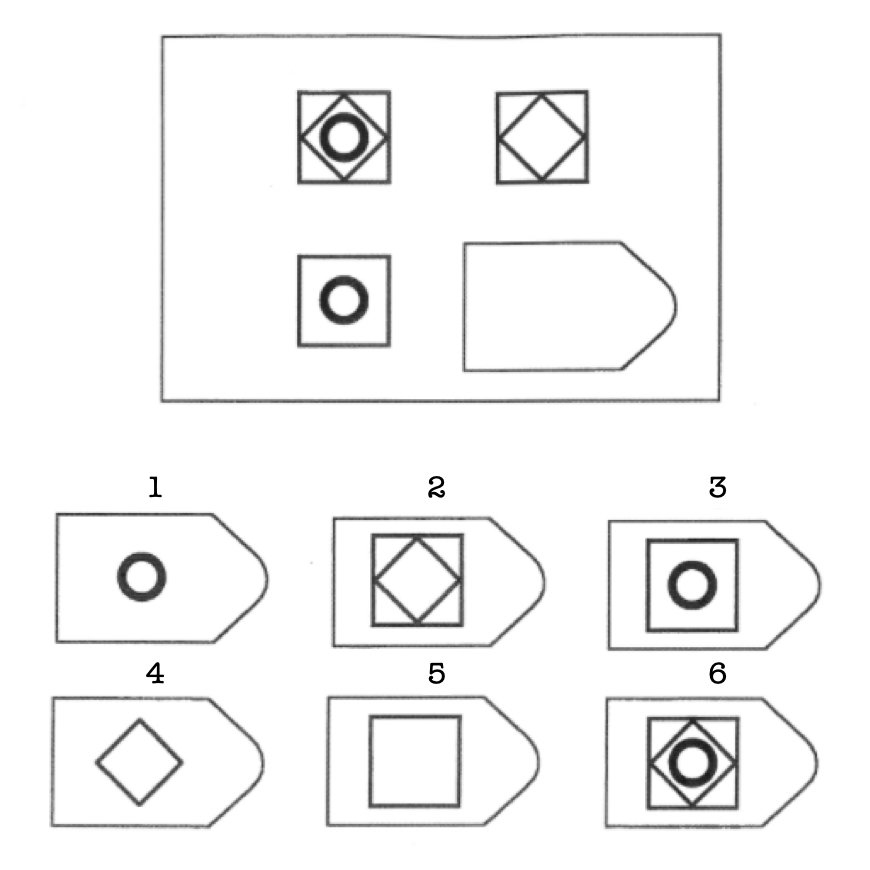
\includegraphics[scale=0.2]{Ravens Survey.jpg}
\end{figure}

\noindent Next, we will present you with a list of the names of all the students in this room. We will ask you to recommend the three people you think will score the highest on the general intelligence test. \\

\noindent If you are chosen by the computer, each of your recommendations in the top 3 increases your chances of winning one of the 100.000 pesos bonuses. \\

\noindent\rule{\textwidth}{0.4pt}\\

\noindent Select the students in this classroom who you consider to have the highest scores on the general intelligence test. (Select 3 students) \\

\noindent [Classroom-specific list of all classmate names visible on one screen. Participants have to pick 3 classmates to continue. Picking their own name invalidates their choices.]\\

\noindent\rule{\textwidth}{0.4pt}\\

\noindent \textbf{Recommendation - Emotions} \\

\noindent All participants took a test where they had to identify the emotion that best described the expression of each image as in the example below. This test is used to measure social skills. \\

\begin{figure}[htbp]
  \centering
  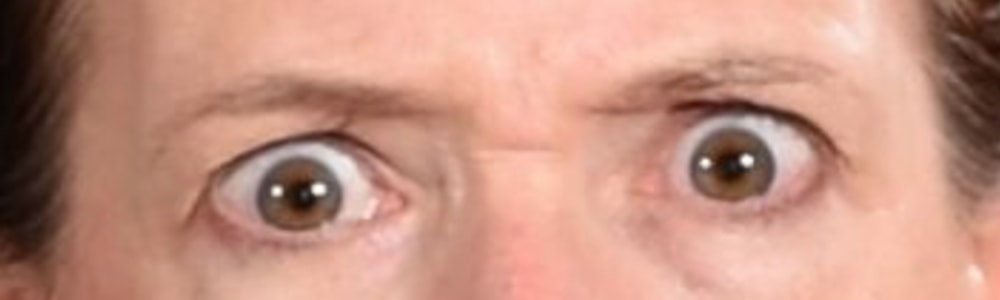
\includegraphics[scale=0.2]{3Aghast-J.jpg}
\end{figure}

\noindent Next, we will present you with a list of the names of all the students in this room. We will ask you to recommend 3 people you think will score the highest on the social skills test. \\

\noindent If you are chosen by the computer, each of your recommendations in the top 3 increases your chances of winning one of the 100.000 pesos bonuses. \\

\noindent\rule{\textwidth}{0.4pt}\\

\noindent Select the students in this classroom who you consider to have the highest scores on the social skills test. (Select 3 students) \\

\noindent [Classroom-specific list of all the names visible on one screen. Participants have to pick 3 classmates to continue. Picking their own name invalidates their choices.]\\

\noindent\rule{\textwidth}{0.4pt}\\

\noindent\textbf{Part 3: Recommendation - Random draw}

\noindent In this part, the computer will randomly choose three students who belong to strata 1, 2, or 3. We will ask you to nominate three people you think the computer will choose. \\

\noindent We will allocate up to [classroom-specific number equal to 20\% of class size] bonuses of 100.000 pesos for Part 3. The steps for allocating the bonuses are explained below. \\

\noindent\rule{\textwidth}{0.4pt}\\

\noindent [classroom-specific illustrations explaining the incentive structure] \\

\begin{figure}[htbp]
  \centering
  \caption{Illustration for the Guessing Task}\label{fig:guessing}
  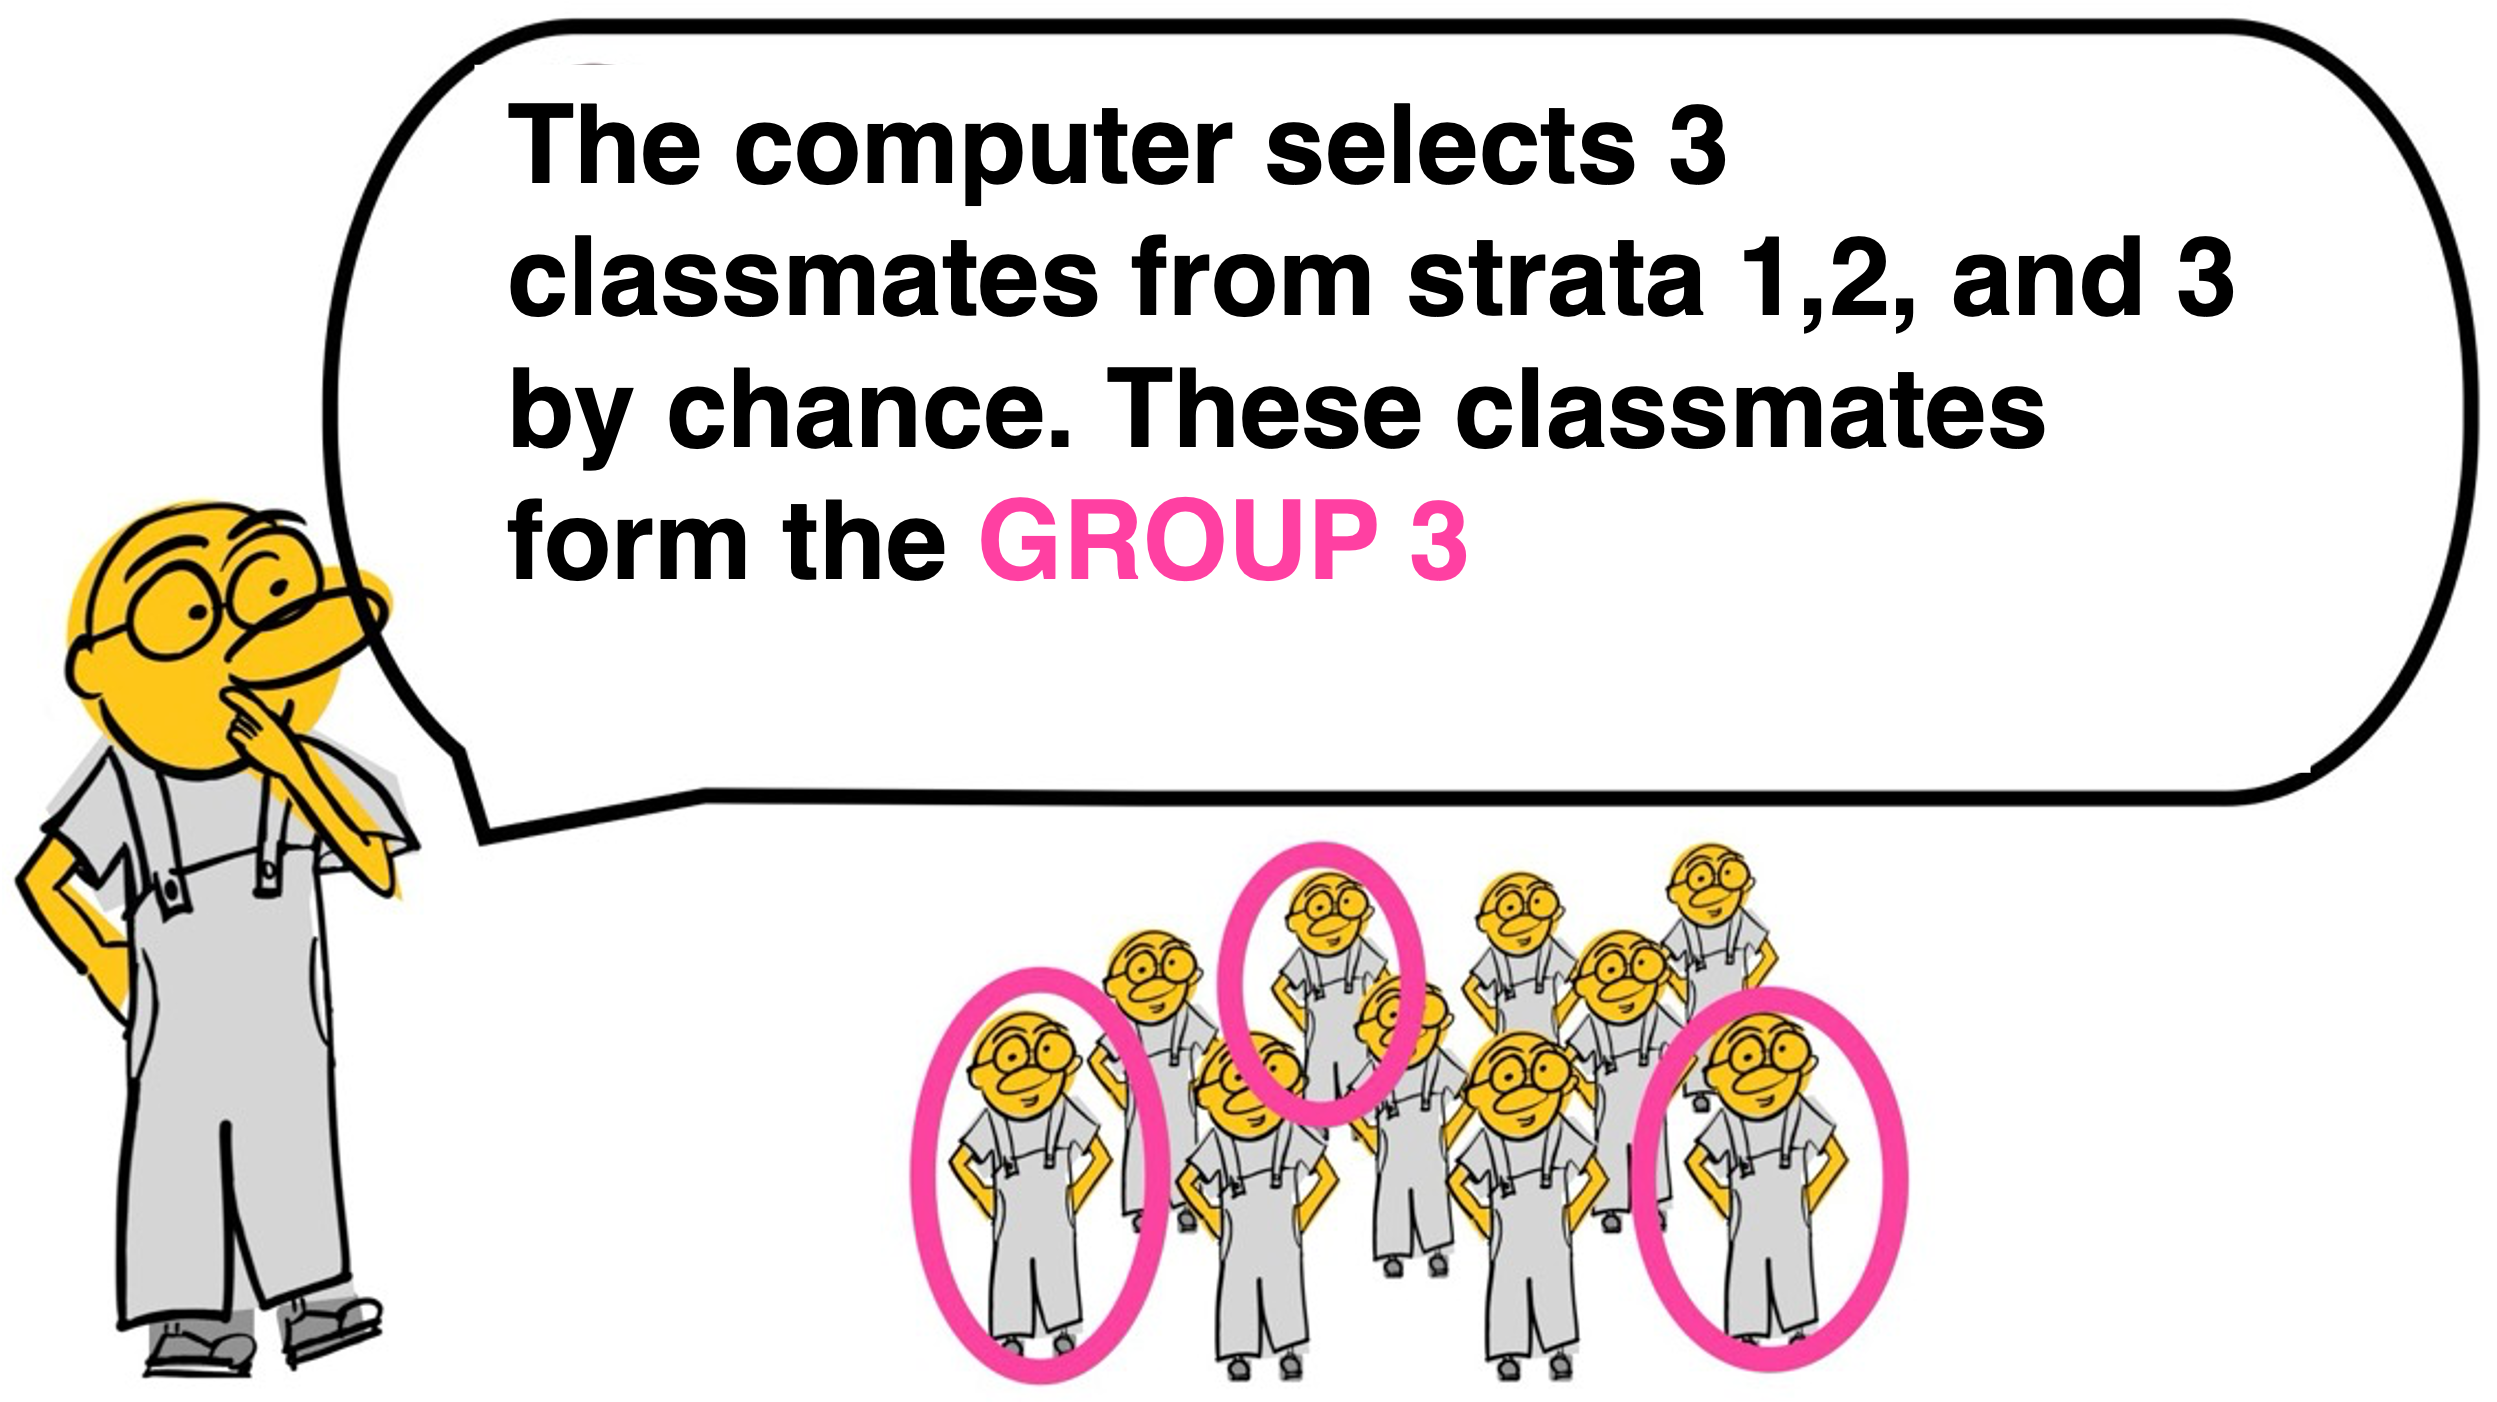
\includegraphics[scale=0.4]{guessing.png}
\end{figure}

\noindent\rule{\textwidth}{0.4pt}\\

\noindent Select the students in this classroom who belong to strata 1, 2, or 3, who you think will be randomly selected by the computer (Select 3 students). \\

\noindent [Classroom-specific list of all the names visible on one screen. Participants have to pick 3 classmates to continue. Picking their own name invalidates their choices.]\\

\noindent\rule{\textwidth}{0.4pt}\\

\noindent \textbf{Part 4}

\noindent Do you want to know your scores on the general intelligence test and the social skills test? We can analyze the data and give you a report that explains your strengths in these two areas. Also, what do these strengths mean, and how can you leverage them for your personal and professional development? \\

\noindent If you want to receive your skills report, we need to contact you again. We also want to be able to invite you to new studies where you can participate for more bonus money. Please indicate if you agree to be contacted again. \\

\noindent [I can be contacted for new studies and to send me my report. I can be contacted to send my report, but not for new studies.  No, I do not want to be contacted again.]

\noindent\rule{\textwidth}{0.4pt}\\

\noindent [if participant gives consent to be contacted again] \\

\noindent Please enter your contact email: \\

\noindent [student email]\\




\end{document}
